\documentclass{report}
% PAGE DIMENSIONS
\usepackage{geometry}
\geometry{a4paper,margin=3.5cm}

% PACKAGES
\usepackage[english]{babel}
\usepackage[T1]{fontenc}
\usepackage[utf8]{inputenc}
\usepackage{graphicx}
\usepackage{fancyhdr}
\usepackage{color}
\usepackage{eso-pic} %background pictures
\IfFileExists{inconsolata.sty}{%Use inconsolata as mono font if available
  \usepackage{inconsolata}
}{}
\usepackage{csquotes}
\usepackage{booktabs}
\usepackage{tabularx}
\usepackage{array}
\usepackage{verbatim}
\usepackage{titlesec}
\usepackage{hyperref}
\usepackage{float}
\usepackage{caption}
\usepackage{subcaption}
\usepackage{amsmath,amsfonts,amssymb,amsthm}
\usepackage{xfrac}
\usepackage[intoc]{nomencl} %for abbreviations list
\usepackage{listings}
\usepackage{marginnote}
\usepackage{url}
\usepackage[normalem]{ulem}
\usepackage{tocbibind}
\usepackage{footnote}

% Bibliography
\usepackage[style=numeric,natbib=true,sortcites=true,block=space,backend=biber]{biblatex}
\bibliography{content/bibliography}
% Use 'biber %' to build bibliography

% marginnote package options
\renewcommand*{\marginfont}{\color{red}\sffamily} %red, sans-serif
\reversemarginpar %margin notes on left side

% listings package settings
\lstloadlanguages{Matlab,[ANSI]C}
\lstset{
  basicstyle=\ttfamily\small,
  %aboveskip=12pt,
  %belowskip=12pt,
  %frame=l,
  numbers=left,
  numberstyle=\ttfamily\tiny,
  numbersep=8pt,
  captionpos=b,
  tabsize=2,
  extendedchars=true,
  breaklines=true,
  showspaces=false,
  showtabs=false,
  keywordstyle=\color{blue},
  escapeinside={(*¤}{¤*)},
  %rangeprefix=,
  %rangesuffix=,
  includerangemarker=false,
  %stringstyle=\color{white}\ttfamily,
  %commentstyle=\color{white} %''cheat'' to hide comments
  xleftmargin=7pt,
  xrightmargin=7pt,
  %backgroundcolor=\color{lightgray},
  showstringspaces=false,
  morekeywords={}
}

% hyperref package settings
\hypersetup{
  unicode=true,          % non-Latin characters in Acrobat’s bookmarks
  pdftoolbar=true,        % show Acrobat’s toolbar?
  pdfmenubar=true,        % show Acrobat’s menu?
  pdffitwindow=false,     % window fit to page when opened
  pdfstartview={FitH},    % fit page to the window Horizontal/Vertical
  pdftitle={TITLE},    % title
  pdfauthor={Alexander Adelholm Brandbyge, Frederik Hagelskjær, Rudi Hansen, Leon Bonde Larsen, Kent Stark Olsen, Kim Lindberg Schwaner},% author
  pdfsubject={SUBJECT},   % subject of the document
  pdfkeywords={wordone} {wordtwo} {SDU}, % list of keywords
  pdfnewwindow=true,      % links in new window
  colorlinks=false,       % false: boxed links; true: colored links
  linkcolor=red,          % color of internal links
  citecolor=green,        % color of links to bibliography
  filecolor=magenta,      % color of file links
  urlcolor=cyan,           % color of external links
  plainpages=false
}

% Widow/orphan penalties
\widowpenalty=300
\clubpenalty=300

% \includegraphics default folder
\graphicspath{{content/graphics/}}

% Float positioning control
\setcounter{topnumber}{2}
\setcounter{bottomnumber}{2}
\setcounter{totalnumber}{3}
\renewcommand{\topfraction}{0.85}
\renewcommand{\bottomfraction}{0.85}
\renewcommand{\textfraction}{0.15}
\renewcommand{\floatpagefraction}{0.4}

% Header colour
\definecolor{FrontpageHeadingColor}{RGB}{5,5,60}%Heading colour definition

% Chapter name formatting
\titleformat
  {\chapter}%command
  [display]%shape
  {\normalfont\huge\bfseries}%format
  {\normalfont\Large\scshape\chaptertitlename\ \huge\thechapter}%label
  {10pt}%sep
  {\Huge}%before

% make nomenclature and change its heading/toc text (see nomencl package)
\makenomenclature
\renewcommand{\nomname}{Abbreviations}
%
%  * Pass this line to MakeIndex:
%    %bm.nlo -s nomencl.ist -o %bm.nls
%
%  * Use \nomenclature{abbr}{discriptive text} to add an entry to the
%    abbreviations list (best done where the abbreviation first occurs in the text)
%  * Example:
%    \nomenclature{ADHD}{Attention Deficit Hyperactivity Disorder}

\begin{document}
%
% Front page
\pagenumbering{alph} %frontpage numbered with a letter
\begin{titlepage}%
\currentpdfbookmark{Front page}{front_page}%hyperref pdf bookmark
%\AddToShipoutPictureBG*{%background picture
% \put(0,0){
%  \parbox[b][\paperheight][b]{\paperwidth}{%\parbox[position][height][inner-pos]{width}{text}
%   \vfill
%   %\begin{flushright}
%   
\includegraphics[width=0.43\paperwidth,trim=110 0 0 0]{content/00_frontmatter/sdu_seal.pdf}%trim=l b r t
%   %\end{flushright}
%   \vspace*{2.9cm}
%  }
% }
%}
\begin{flushright}

\includegraphics[scale=0.73]{content/00_frontmatter/sdu_logo.pdf}
\end{flushright}
\vspace*{2.7cm}
%
%\textsf{\Large{\textbf{Gruppe 1}}}
%
%\vspace*{0.3cm}
\setlength{\extrarowheight}{1.5pt}
\begin{tabular}{@{}l l}
	\textsf{\large{311289}} & \textsf{\large{Alexander Adelholm Brandbyge}}\\
	\textsf{\large{251289}} & \textsf{\large{Frederik Hagelskj�r}}\\
	\textsf{\large{260387}} & \textsf{\large{Rudi Hansen}}\\
	\textsf{\large{150179}} & \textsf{\large{Leon Bonde Larsen}}\\
	\textsf{\large{040282}} & \textsf{\large{Kent Stark Olsen}}\\
	\textsf{\large{160788}} & \textsf{\large{Kim Lindberg Schwaner}}
\end{tabular}
\setlength{\extrarowheight}{0pt}
\vspace*{1.5cm}
\\
\textsf{\Huge{\textbf{\textcolor{FrontpageHeadingColor}{Overskrift}}}}
\vspace*{0.5cm}
\\
\textsf{\Large{\textbf{\textcolor{FrontpageHeadingColor}{Underoverskrift}}}}
\vfill
\textsf{\\Faculty of Engineering\\
University of Southern Denmark\\
Niels Bohrs All� 1\\
5230 Odense M\\
Denmark}
\vspace*{10pt}
\\
\textsf{www.sdu.dk/tek\\
+45 6550 7303\\
tek@tek.sdu.dk}
\end{titlepage}%

%
% Abstract (un-numbered chapter)
\pagenumbering{roman} %until main content we use roman page numbering
\chapter*{Abstract}\addcontentsline{toc}{chapter}{Abstract}

The purpose of this project is to create a pan-tilt device, which position is to be regulated. A model of the pan-tilt system will be developed and a regulation system will be created for it. The device is moved by two dc motors, which are controlled by a FPGA, which also tracks speed and position. The system is regulated by an ARM microprocessor and the ARM is also taking care of the user interface. The ARM is programmed in C and a FreeRTOS OS is running on the system. The two units are communicating by a SPI connection. The team decided to divide the project into small independent modules. This will result in a high cohesion which will make modifications much easier to implement and earlier developed modules can be reused in the development, debugging and testing of other modules.

This report will include the analyses and solutions to the challenges that the individual modules will create.

Lidt ekstra der skal tilføjes

The user interface will be developed in intent of showing the systems capabilities in regulating the pan-tilts position.
The FPGA is a Spartan3E which will be programmed in VHDL. 
%
% Preface (un-numbered chapter)
\chapter*{Preface}\addcontentsline{toc}{chapter}{Preface}
Wee

%
% Table of contents, figures, tables, listings and abbreviations
\tableofcontents
\listoffigures
\listoftables
\lstlistoflistings\addcontentsline{toc}{chapter}{Listings}
\printnomenclature[1.5cm]
%
% MAIN CONTENT
\clearpage
\pagenumbering{arabic} %''normal'' arabic numbering from here on out
%
\chapter{Introduction}\label{chap:intro}

This project is devised as a part of the B.Sc. Robot Systems Engineering, 4th term course at the Faculty of Engineering, University of Southern Denmark, Odense spring 2012. The implicit goal is to obtain basic knowledge of embedded systems. This is because embedded systems figure as a significant part of robots as these systems often controls actuators and process sensor inputs for controlling the robot. Therefore it is also demanded for students participating in this course to grasp the basic concepts of control theory. Coupling control theory and embedded systems demand understanding of the basics of real time systems, digital systems, embedded systems and control systems. Applying this knowledge in the real world will be as significant as grasping the concepts.

Because the DSMI\footnote{The Engineering Education Model of the University of Southern Denmark} model is used as a framework for this particular education, it is required for the students participating in this course to formulate a strategy for solving an assignment in teams.

\section{Project description}
The purpose of the project work is to construct a control system for the pan/tilt frame shown in figure \ref{fig:pantiltsystem}, so that it is possible to control it with one or more user inputs. For example a joystick, a keyboard, buttons or by commands from a computer. In addition the system should also provide the user with options for feedback of significant system parameters. This is to be prioritized in the project:
\begin{itemize}
  \item A system analysis and modelling of the individual elements of the system.
  \item Analysis and design of the regulation loops in Matlab and Simulink.
  \item Documentation of FPGA design and implementation.
  \item Documentation of the design and implementation of microprocessor program, including choice of operating system.
  \item Test and verification of the system.
\end{itemize}



It is up to the project group to choose the characteristics of the regulator system and the regulator loops.

\begin{figure}[htb]
	\centering
	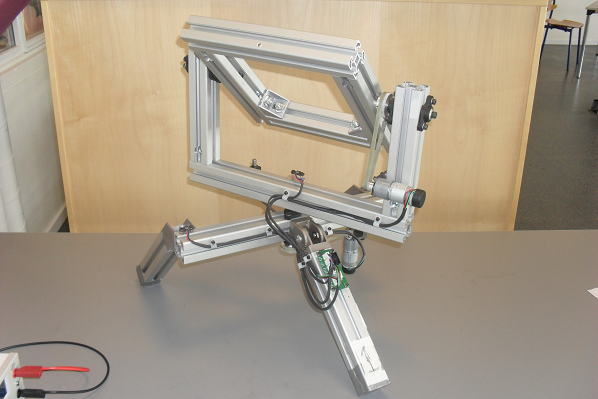
\includegraphics[width=\textwidth]{graphics/pantiltsystem.png} %trim=l b r t
	\caption{The pan/tilt system.}
	\label{fig:pantiltsystem}
\end{figure}

\pagebreak
\section{Requirements}
The following conditions are set for the system:
\begin{itemize}
\item The controller must be implemented on a microprocessor.
\item SPI must be used as the method of communication between the microprocessor and the FPGA.
\item The FPGA must control the PWM signals to the motors.
\item The FPGA must be used to determine the motors positions through use of  their built-in encoders.
\end{itemize}
%\usepackage{graphicx}

\section{Project description}
The purpose with the project work is to construct a Pan and Tilt system, for the  shown in figure \ref{fig:pantilysystem}, so that it is possible to control the system from one or more user inputs eg a joystick, a keyboard, buttons or via commands from a computer. In addition shall the system also give the user options for feedback of significant system parameters.

\begin{figure}[htb]
	\begin{center}
	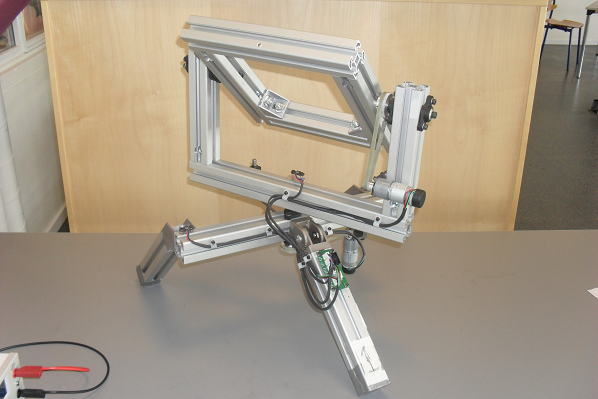
\includegraphics[scale=1,trim=0 0 0 0]{graphics/pantiltsystem.png} %trim=l b r t (can cut off from every side)
	\caption{The given pant tilt system.}
	\label{fig:pantilysystem}			% figure labels are of the form \label{fig:*}
	\end{center}
\end{figure}

\begin{itemize}
\item A system analysis and modulation of the systems individual elements.
\item Analysis and design of the regulation loops in Matlab and Simulink.
\item Documentation of FPGA design and implementation.
\item Documentation of the microprocessor programs design and implementation, including division into tasks and selection of scheduling.
\item Test and verification of the system.
\end{itemize}

It is up to the project group to chose the regulator system og the regulator loops' characteristics.

\section{Requirements}

The following conditions are set for the system:
\begin{itemize}
\item The regulators' must be implemented on a microprocessor.
\item SPI must be used in communication between the microprocessor and the FPGA.
\item The FPGA shall control the PWM signals to the motors.
\item The FPGA shall be used to determine the motors position via the encoders.
\end{itemize}

\section{The physical system}

The following is provided for the project:

\begin{itemize}
\item 2 pc. Pan and Tilt setup, that is to be shared between the project groups.
\item Motor with built in encoder to every project group.
\item Print with double H-bridge to every project group.
\end{itemize}

For the rest of the system the following devices are used:

\begin{itemize}
\item The microprocessor is a Stellaris LM3S6965 on an Evaluation Board, which is mounted on a test board with keypad, incremental rotary encoder, potentiometer and an LCD.
\item All hardware for user interface is from the given ARM test board.
\item The FPGA is a Xilinx Nexys 2 board with a Spartan-3E chip on board.
\item The SPI connection is made by connecting wires between ports on the to boards.
\end{itemize}

The pysical system was set up as following as shown in figure \ref{fig:digitalsystem}. All the user interface mounted with the microprocessor, all the motor input and output at the FPGA and a SPI connection between the two:

\begin{figure}[htb]
	\begin{center}
	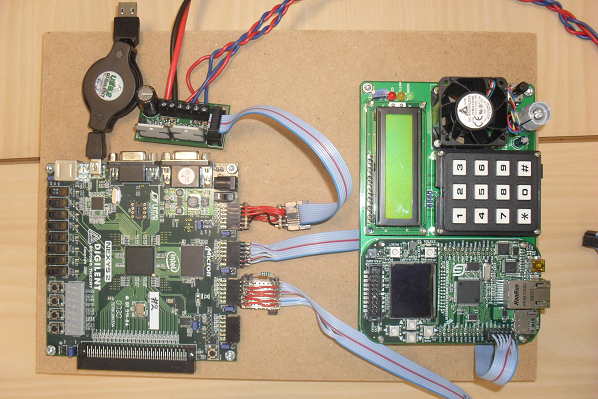
\includegraphics[scale=1,trim=0 0 0 0]{graphics/digitalsystem.png} %trim=l b r t (can cut off from every side)
	\caption{Setup of the electrical system.}
	\label{fig:digitalsystem}			% figure labels are of the form \label{fig:*}
	\end{center}
\end{figure}

\section{Complete system}

The complete system is shown in figure \ref{fig:completesystem}, here are all individual components that need to be created for the system. The exact number of tasks is not meant to be shown, but as a reference to understand the analysis of the system.

(Diagrammet skal aendres!)

Meningen er at der skal være en lille analyse af hvad der skal udvikles/ hvordan systemet skal se ud...


\begin{figure}[htb]
	\begin{center}
	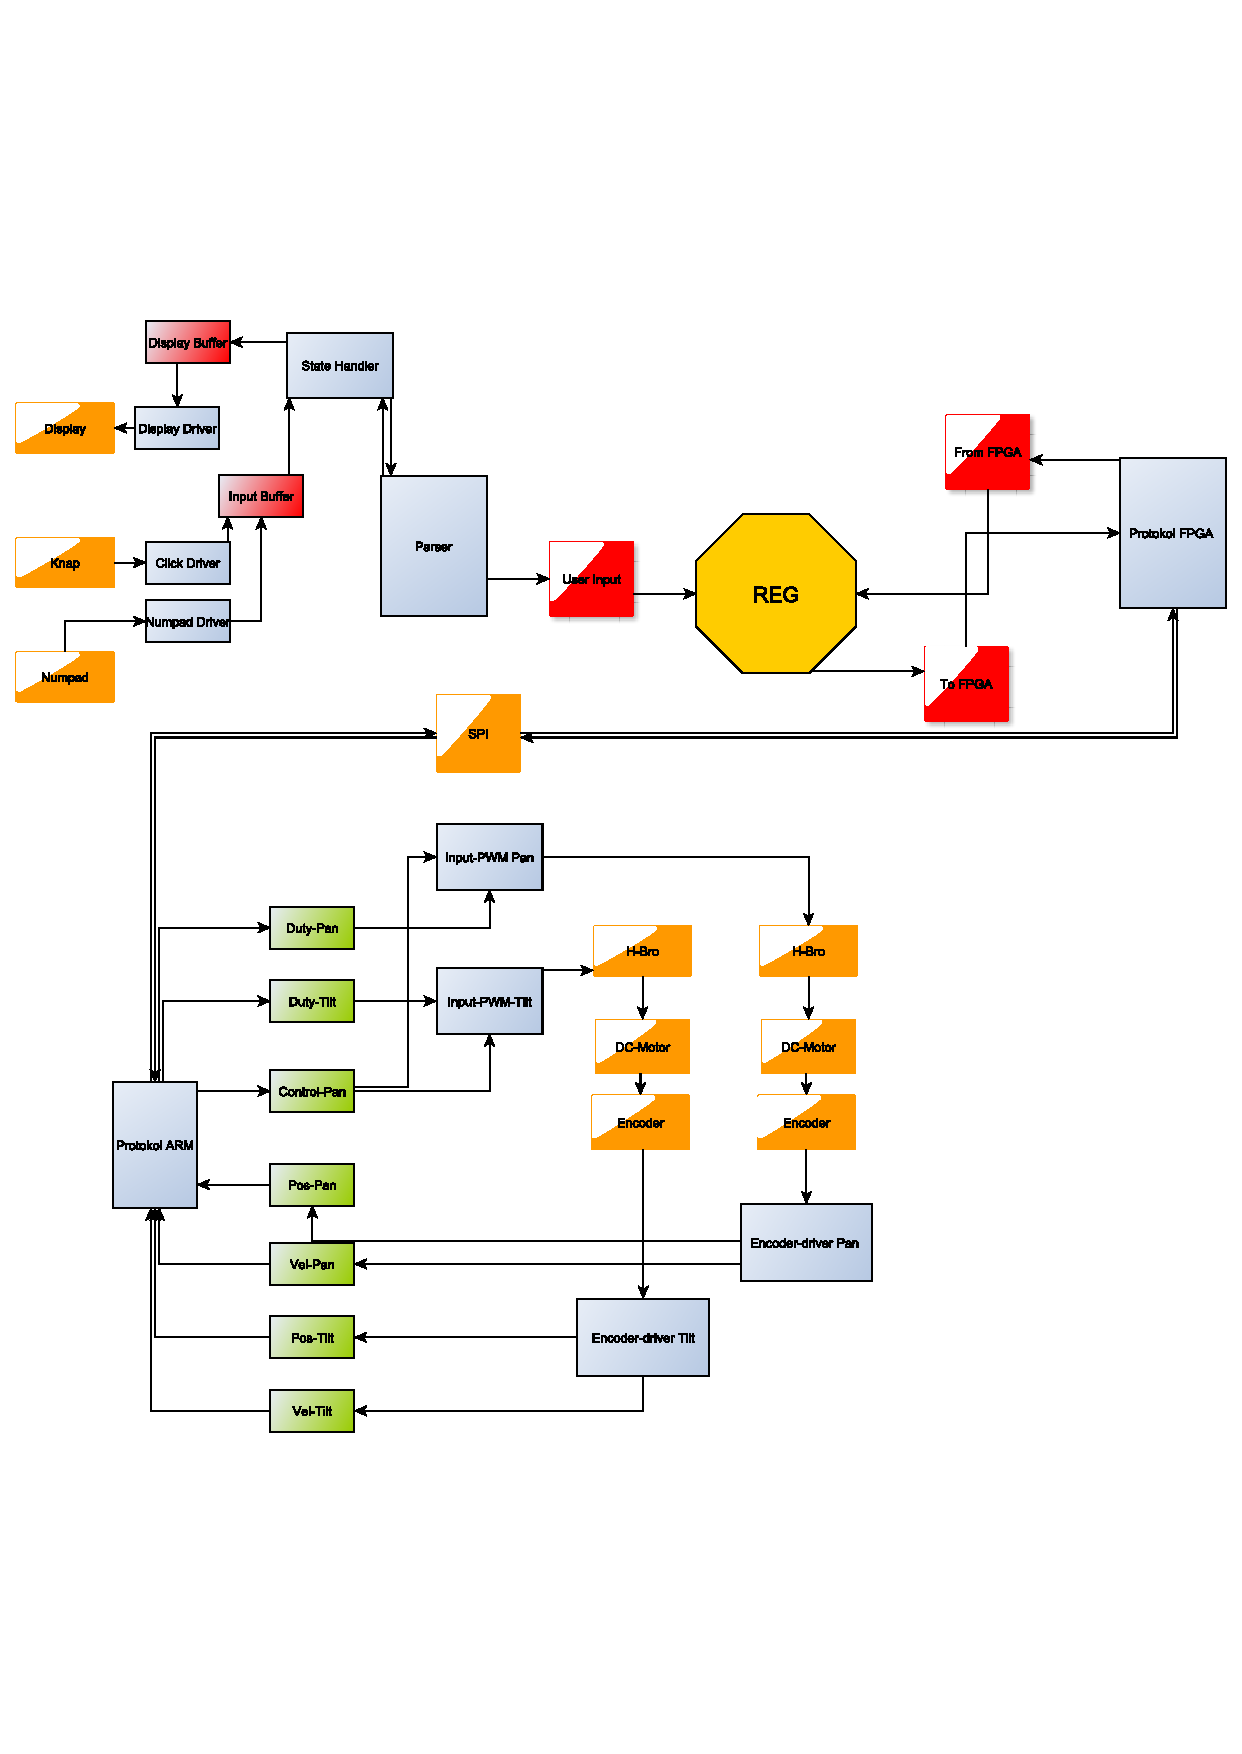
\includegraphics[scale=0.8,trim=100 130 100 250]{graphics/Project4GreaterPresentation3.pdf} %trim=l b r t (can cut off from every side)
	\caption{Setup of the complete system. Orange are physical components. Red are variables. Blue are tasks. Green are RAM. }
	\label{fig:completesystem}			% figure labels are of the form \label{fig:*}
	\end{center}
\end{figure}
\chapter{Dynamics}\label{chap:dynamics}
This chapter will contain an analysis of the dynamics of the pan/tilt system which will result in a mathematical model. Calculations made throughout this chapter will reside in appendix \ref{app:dynamics_calc}. Identifying and understanding the relevant dynamics of a system is important as this will lead to an as accurate theoretical model as needed for the application. Ideally a perfect model would somewhat be preferred, but it would be a very difficult and tedious task to derive a perfect model and completely unnecessary to achieve. The reason for that is some of the dynamics are completely insignificant to the behaviour of the system, some others might have a little impact on the behaviour but can be omitted due to more dominating dynamic. The response of electrical circuits are often much quicker than the response of a mechanical system. This response delay is encoded into the poles of a system, which makes the poles of the system very interesting to analyse. The poles of the system tell if it is stable, and if any dynamic in the system possibly can be omitted due to its relatively fast response compared to the rest of the system which acts slower.

Every system can be constructed of first order systems and second order systems in a cascade. These two types of systems defines a time constant. For first order systems this time constant is hidden in the zeroth order term and in second order systems it is hidden in the first order term. From a physical point of view the time constant defines the point in time where the system reaches $1 - \sfrac{1}{e} \approx 63.2\%$ of its final energy state, below in figure \ref{fig:energy_systems} is illustrated a step response on a first and a second order system.
\begin{figure}[htb]
	\begin{center}
	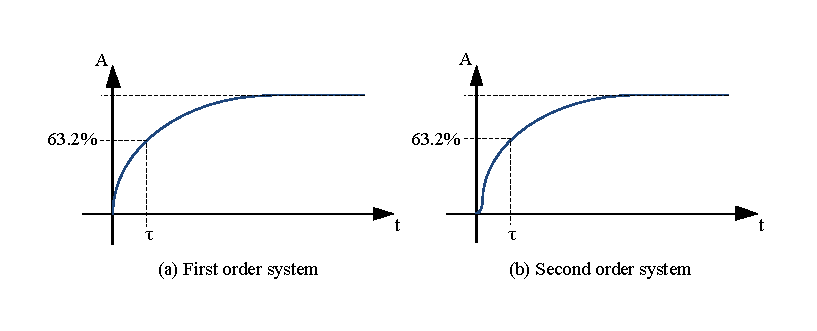
\includegraphics[scale=1,trim=0 0 0 0]{graphics/energy_systems.pdf} %trim=l b r t (can cut off from every side)
	\caption{(a) Illustrates the step response of a first order system. (b) Illustrates a step response of a second order system. Both will raise in time and reach some asymptotic value provided that the systems are stable, $\tau$ denotes the time constant.}
	\label{fig:energy_systems}			% figure labels are of the form \label{fig:*}
	\end{center}
\end{figure}
In figure \ref{fig:energy_systems}(b), notice the transient which seems more inert compared to (a). This is due to some mass in the system if the second order differential equation which represents the system is a mechanical equation. The transient response of a system is encoded into the poles of the system, which is defined by the time constant the following way:
\begin{equation}
	\tau = \frac{1}{\zeta\omega_{n}}\label{eq:time_constant}
\end{equation}
where $\zeta$ is the dampening ratio and $\omega_{n}$ is the undampened natural frequency, this relates to the poles as seen in figure \ref{fig:s_plane}.
\begin{figure}[htb]
	\begin{center}
	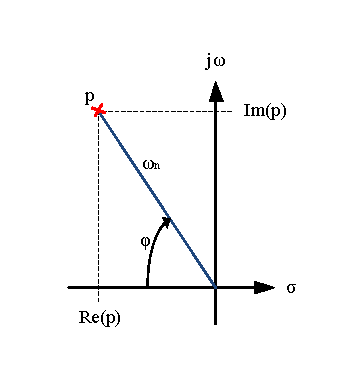
\includegraphics[scale=1,trim=0 0 0 0]{graphics/splane.pdf} %trim=l b r t (can cut off from every side)
	\caption{This figure illustrates a pole in the s-plane and the relation between poles and time constants.}
	\label{fig:s_plane}			% figure labels are of the form \label{fig:*}
	\end{center}
\end{figure}
In figure \ref{fig:s_plane} the real part of the pole is given by $Re(p) = - \zeta\omega_{n} = - \omega_{n} \cos(\varphi)$ and the imaginary part is given by $Im(p) = j\omega_{n}\sqrt{1 - \zeta^{2}} = j\omega_{n}\sin(\varphi)$. Considering equation \ref{eq:time_constant} and figure \ref{fig:s_plane} it is easy to see that real part of a pole directly relates to the time constant. Systems with one pole can therefore have their time constant calculated from the poles real part. Systems consisting of more than one pole can have their time constant calculated from the super positioning the poles real part. Below is shown an example.
\begin{equation}
	\tau = \frac{1}{Re(p_{1})} + \frac{1}{Re(p_{2})} + \frac{1}{Re(p_{3})} + ...\label{eq:time_constant}
\end{equation}
As the time constant is defined as the reciprocal of the real part of the pole, then poles far away from the imaginary axis will not add that much to the total time constant as poles located near the imaginary axis. Therefore can the following be concluded, \textit{faster} poles in a system compared to \textit{slower} poles can be omitted from the model of the system.

\section{Overview of pan/tilt}
The following will give an overview of the physical aspects of the pan/tilt system and also define the mathematics which is tied to the system. The pan/tilt is assembled from two motors, a set of gears connected to each motor. Each motor can rotate a mass individually by transferring torque from the motors, through the gears, to the masses which are connected to the gears. A model of the motors are needed, along with a model of the reflected inertia through the gears, and other dynamics might be relevant to, but are discussed later in this section.

\subsection{Motor}
The motor converts electrical energy to mechanical energy as a voltage is supplied to the motor. This voltage make the motor turn and this turning motion deliver torque though some gears to a mass which then spins up to some maximum speed. A simplification of a DC motors circuit can be seen in figure \ref{fig:motor_circuit}, from this a mathematical model of the motor can be derived.
\begin{figure}[htb]
	\begin{center}
	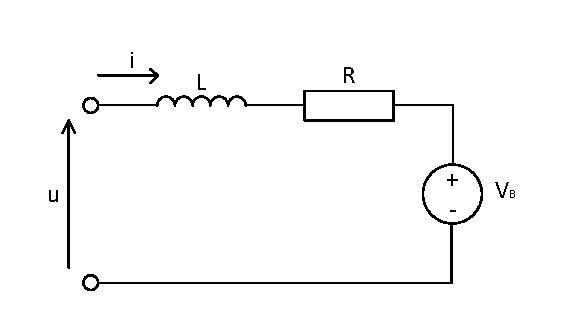
\includegraphics[scale=1,trim=0 0 0 0]{graphics/motor_circuit.pdf} %trim=l b r t (can cut off from every side)
	\caption{Simplification of circuit for a DC motor. Voltage supplied is denoted by $u$, $i$ is the current through the motor, $L$ is inductance, $R$ is resistance and $V_B$ is the the voltage generated from the coil rotating in a magnetic field.}
	\label{fig:motor_circuit}			% figure labels are of the form \label{fig:*}
	\end{center}
\end{figure}
Following can be derived from the circuit seen in figure \ref{fig:motor_circuit}.
\begin{align}
	u &= L\frac{di}{dt} +  Ri + V_B \Longleftrightarrow\\
	u &= L\frac{di}{dt} +  Ri + K_B\omega\label{eq:motor_model}
\end{align}
where $u$ is the voltage input, $i$ is the current, $\frac{di}{dt}$ is the time derivative of the current, $L$ is the inductance, $R$ is the resistance and $V_B$ is the voltage generated in the in coil of the motor as it spins in a magnetic field. $V_B$ can be expressed by $K_B$ which is the \textit{back-emf}\footnote{EMF is an abbreviation for electromotive force, which is the voltage generated from a coil rotating in a magnetic field.}-constant, times $\omega$, which is the angular velocity of the motor. As the motors need to move a mass an expression for torque is more interesting compared to the expression derived in \ref{eq:motor_model}. The electrical torque can be expressed in the following way:
\begin{equation}
	\tau = K_Ti\label{eq:electrical_torque}
\end{equation}
where $K_T$ is the torque constant.	The mechanical torque can be expressed in the following way:
\begin{equation}
	\tau = J_L\frac{d\omega}{dt}\label{eq:mechanical_torque}
\end{equation}
where $J_L$ is the inertial load on the motor, $\frac{d\omega}{dt}$ is the time derivative of the angular velocity of the motor. Equation \ref{eq:electrical_torque} and \ref{eq:mechanical_torque} equals each other if it is assumed that the energy is conserved in the transfer from electrical to mechanical torque, the following expression is obtained then obtained from equation \ref{eq:electrical_torque} and \ref{eq:mechanical_torque}:
\begin{align}
	K_Ti &= J_L\frac{d\omega}{dt} \Leftrightarrow\\
	i &= \frac{J_L}{K_T} \frac{d\omega}{dt}\label{eq:electrical_mechanical_torque}
\end{align}
To derive $\frac{di}{dt}$ the time derivative is taken of \ref{eq:electrical_mechanical_torque} which leads to:
\begin{equation}
	\frac{di}{dt} = \frac{J_L}{K_T} \frac{d^{2}\omega}{dt^{2}}\label{eq:electrical_mechanical_torque_derivative}
\end{equation}
Now \ref{eq:electrical_mechanical_torque} and \ref{eq:electrical_mechanical_torque_derivative} can be substituted into \ref{eq:motor_model} in which the following is obtained:
\begin{equation}
	u = \frac{L J_L}{K_T} \frac{d^{2}\omega}{dt^{2}} + \frac{R J_L}{K_T} \frac{d\omega}{dt} + K_B \omega\label{eq:model_model}
\end{equation}

Stiction, coulomb and viscous friction are omitted as it is assumed that the inertia from the internal friction of the motor is a lot less than the inertia from the mass, so this concludes the model of the motor.

\subsection{Gears}
The gears between the mass to be rotated and the motor of the system reflect the actual inertia of the mass onto the motor. Calculations for the reflected inertia is kept in appendix \ref{app:dynamics_calc}.
  
\subsection{Torque-induced precession}
When a body rotates around an axis the phenomenon of precession occurs. The torque-induced precession occurs when a body accelerates around an axis a torque is induced perpendicular to the axis of rotation. In figure \ref{fig:precession} a sketch of this situation is shown.
\begin{figure}[htb]
	\begin{center}
	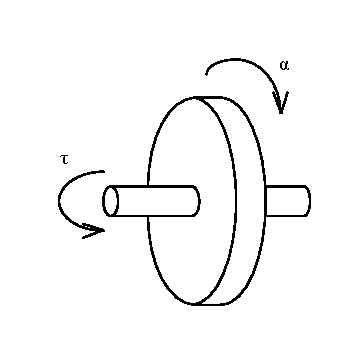
\includegraphics[scale=1,trim=0 0 0 0]{graphics/precession.pdf} %trim=l b r t (can cut off from every side)
	\caption{Show the concept of of the torque-induced precession.}
	\label{fig:precession}			% figure labels are of the form \label{fig:*}
	\end{center}
\end{figure}
This torque is given by:
\begin{equation}
	\tau = I\alpha\label{eq:induced_torque}
\end{equation}
where $\tau$ is the torque, I is the inertia of the body rotating and $\alpha$ is the angle acceleration the body is affect by. An example is that if the tilt part of the system is accelerating up to some velocity, a torque will be applied to the pan part of the system, this torque is acting perpendicular to the rotation causing the pan to rotate as long as the motor for the tilt part is accelerating. To investigate the impact of the torque-induced precession, equation \ref{eq:motor_model} and \ref{eq:induced_torque} have to be related to each other. As equation \ref{eq:induced_torque} is expressed as torque, equation \ref{eq:motor_model} is rewritten with respect to torque, equation \ref{eq:mechanical_torque}.
\begin{equation}
	J_L \frac{d\omega}{dt} = \frac{K_T}{R} u - \frac{L J_L}{R} \frac{d^{2}\omega}{dt^{2}} - \frac{K_B K_T}{R} \omega\label{eq:torque_motor_model}
\end{equation}
then equation \ref{eq:induced_torque} is subtracted from the total torque \ref{eq:torque_motor_model} as follows:
\begin{equation}
	J_L \frac{d\omega_{1}}{dt} = \frac{K_T}{R} u - \frac{L J_L}{R} \frac{d^{2}\omega_{1}}{dt^{2}} - \frac{K_B K_T}{R} \omega_{1} - I \frac{d\omega_{2}}{dt}\label{eq:coupled_torque_motor_model}
\end{equation}
where $\omega_1$ for example is the velocity of the pan and $\omega_2$ is the velocity of the tilt. 

\section{Finding parameters}
The following will contain a brief discussion on how the parameters was found. To obtain the parameters for the model some measurements where made on tilt part of the system, these measurements and the Matlab script which was used for analysing the data is located on the CD. The measurements that where produced is expressed in position $[ticks]$ against time $[ms]$. All the previous equations are dependent of the velocity of the system, so the measurements have to be differentiated with respect to time, this is done by a numerical method called the secant method\footnote{NR ref}, the differentiated result is plotted and shown in figure \ref{fig:measured_step_tilt}.
\begin{figure}[htb]
	\begin{center}
	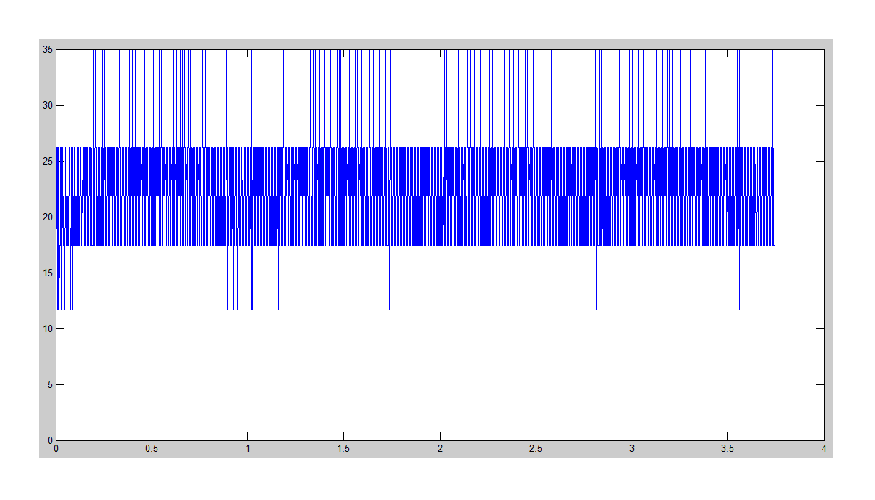
\includegraphics[scale=1,trim=0 0 0 0]{graphics/measured_step_tilt.pdf} %trim=l b r t (can cut off from every side)
	\caption{This graph show the actual velocity of the tilt part of the system. The horizontal axis show time in seconds. The vertical axis show angular velocity in radians per second.}
	\label{fig:measured_step_tilt}			% figure labels are of the form \label{fig:*}
	\end{center}
\end{figure}
If a mean is calculated from the steady-state part of the graph $22.57 \sfrac{rad}{s}$ is obtained, and compared to the data sheet of the motor which says the rated speed is $22.62 \sfrac{rad}{s}$, the data from the graph represented in figure \ref{fig:measured_step_tilt} is assumed to be correct. Next a set of equations are formed from equation \ref{eq:model_model}, the input is set to zero and rewritten as follows:
\begin{equation}
	\frac{d^{2}\omega}{dt^{2}} = - \frac{R}{L} \frac{d\omega}{dt} - \frac{K_B K_T}{L J_L} \omega
\end{equation}
where $\frac{d^{2}\omega}{dt^{2}}$, $\frac{d\omega}{dt}$, and $\omega$ is known, this is due to that these can be calculated with numerical analysis, so the constants $\frac{R}{L}$ and $\frac{K_B K_T}{L J_L}$ can be found. $R$ and $J_L$ is also known and $K_B = K_T$. Matlab have been used for calculating the set of equations $\textbf{Ax} = \textbf{b}$, so that the rest of the unknowns can be found. Check Matlab script located on the CD to see further details about how the set of equations where formed.

\subsection{Verification}
Previous experiments and calculations have shown that $R = 5.124\Omega$, $L = 38.4mH$ and $K_B = K_T = 35.1 \sfrac{mV}{\dfrac{rad}{s}}$. Through the Matlab script included on the CD, $\frac{R}{L}$ and $\frac{K_B K_T}{L J_L}$ is found to be the following:
\begin{equation}
	\frac{R}{L} = 791.7 \Rightarrow L = \frac{5.124}{791.7} \approx 6.471mH
\end{equation}
\begin{equation}
	\frac{K_B K_T}{L J_L} = 25.63\label{eq:constants}
\end{equation}
According to equation \ref{app:eq_reflected_pan_inertia}, $J_L = 0.970 \cdot 10^{-3} kg \cdot m^{2}$ which is the reflected inertia of the tilt part through the gears, $L = 6.471mH$, and $K_B = K_T$. Now $K_B$ and $K_T$ can be calculated the following way:
\begin{equation}
	K_B = K_T = \sqrt{25.63 \cdot L \cdot J_L} \Rightarrow K_B = K_T = \sqrt{25.63 \cdot L \cdot J_L} \approx 401.1 \frac{mV}{\sfrac{rad}{s}}
\end{equation}
Compared to the values found in previous experiments the values found here does not match, so which parameters to use? This can be answered by looking at a pole-zero plot of the system and the open-loop response of the system. To set up the model a state-space representation is made of the system as follows below. The coupled system is set up with respect to equation \ref{eq:coupled_torque_motor_model}:

\begin{array}{•}

\end{array}

%%%%%%%%%%%%%%%%%%%%%%%%%%%%%%%%%%%%%%%%
%% Kblet MODEL hEr og nu, men helst i går




\chapter{Control system}\label{chap:control_system}
\section{Designing a regulator}
This chapter concerns implementation of a regulator for the pan tilt system. So
far the system has been analyzed as open loop and no feedback has considered.
The objective in designing this controller is to increase the performance of the
system, in this case meaning to track a position. 

\subsection{Requirements}
In the dynamics chapter it was concluded that a decoupled model of the system is
sufficient and therefore a regulator for pan part and a regulator for the tilt
part can be designed individually.

The controller is developed focusing mainly on optimizing the precision and less
on optimizing speed and settling time. Therefore the objective is to design a
regulator with a steady state error of zero. This is in therory done by adding
an integrator, to raise the type of the system, so at least the regulatior should be of type PI.

\subsection{Design}
SISO\footnote{Single input, single output}-control systems can be sketched the
following way:
\begin{figure}[htb] \centering 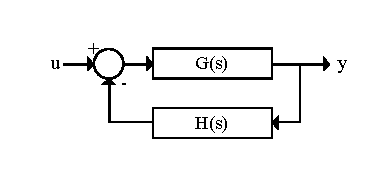
\includegraphics[width=\textwidth,trim=0 0 0
0]{graphics/control_sketch.pdf} %trim=l b r t (can cut off from every side)
	\caption{This figure illustrates a sketch of a general control system.}
	\label{fig:control_sketch}			% figure labels are of the form \label{fig:*}
\end{figure}
Figure \ref{fig:control_sketch} show a system with a feedback loop, $G(s)$ is
the plant and $H(s)$ is the regulator. When designing a regulator ($H(s)$) is
derived and since the system is SISO, a PID regulator can be designed.

\subsection{PID parameters}
A PID regulator can be expressed in the following way:
\begin{equation}
	h(t) = K_p e(t) + K_i \int\limits_0^t e(\tau) d\tau + K_d \frac{de(t)}{dt}
\end{equation}
where $K_p$, $K_i$, and $K_d$ are constants for the proportional, integral, and differential term in the equation. Applying LaPlace-transform leads to:
\begin{equation}
	H(s) = E(s)(K_p + \frac{K_i}{s} + K_d s)
\end{equation}
Though various methods are available for deriving the optimal parameters, the
approach chosen here is to do a mathematical simulation of the system. Since the
transfer functions have already been derived, a Simulink model can be developed.

Since the system is decoupled, it can be represented as shown in figure \ref{fig:control_sketch} \begin{figure}[htb]
	\centering
	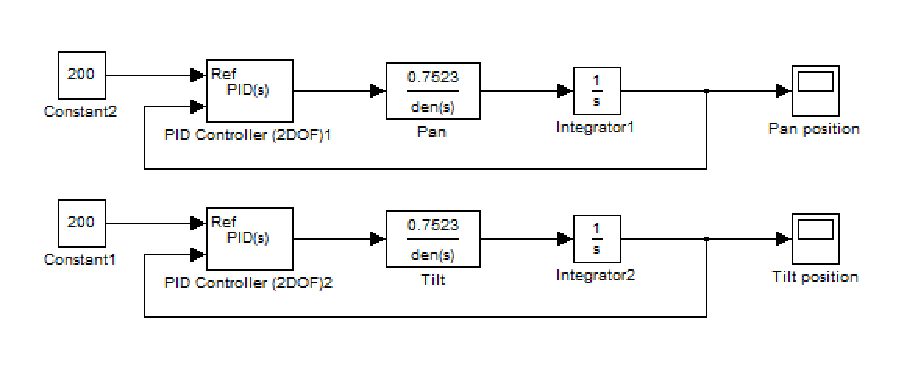
\includegraphics[width=\textwidth,trim=0 0 0 0]{graphics/Simulink.pdf} %trim=l b r t (can cut off from every side)
	\caption{This figure illustrates the simulink model.}
	\label{fig:control_sketch}			% figure labels are of the form \label{fig:*}
\end{figure}
The top system represent the pan part of the system, while the lower part represent the tilt.

\subsection{Simulation}
The goal of the simulation is to find the values providing a qickly responding system, while still remaining stable and robust. To obtain a first guess of the P-term, the root locus method is applied. The root locus plot can be seen in figure \ref{fig:rlocus_plot}. Aiming to minimize the energy needed to move the system, equal magnitudes of real and imaginary parts are chosen, leading to the base gain denoted in table \ref{tab:gain_values}.

\begin{figure}[htb]
	\centering
	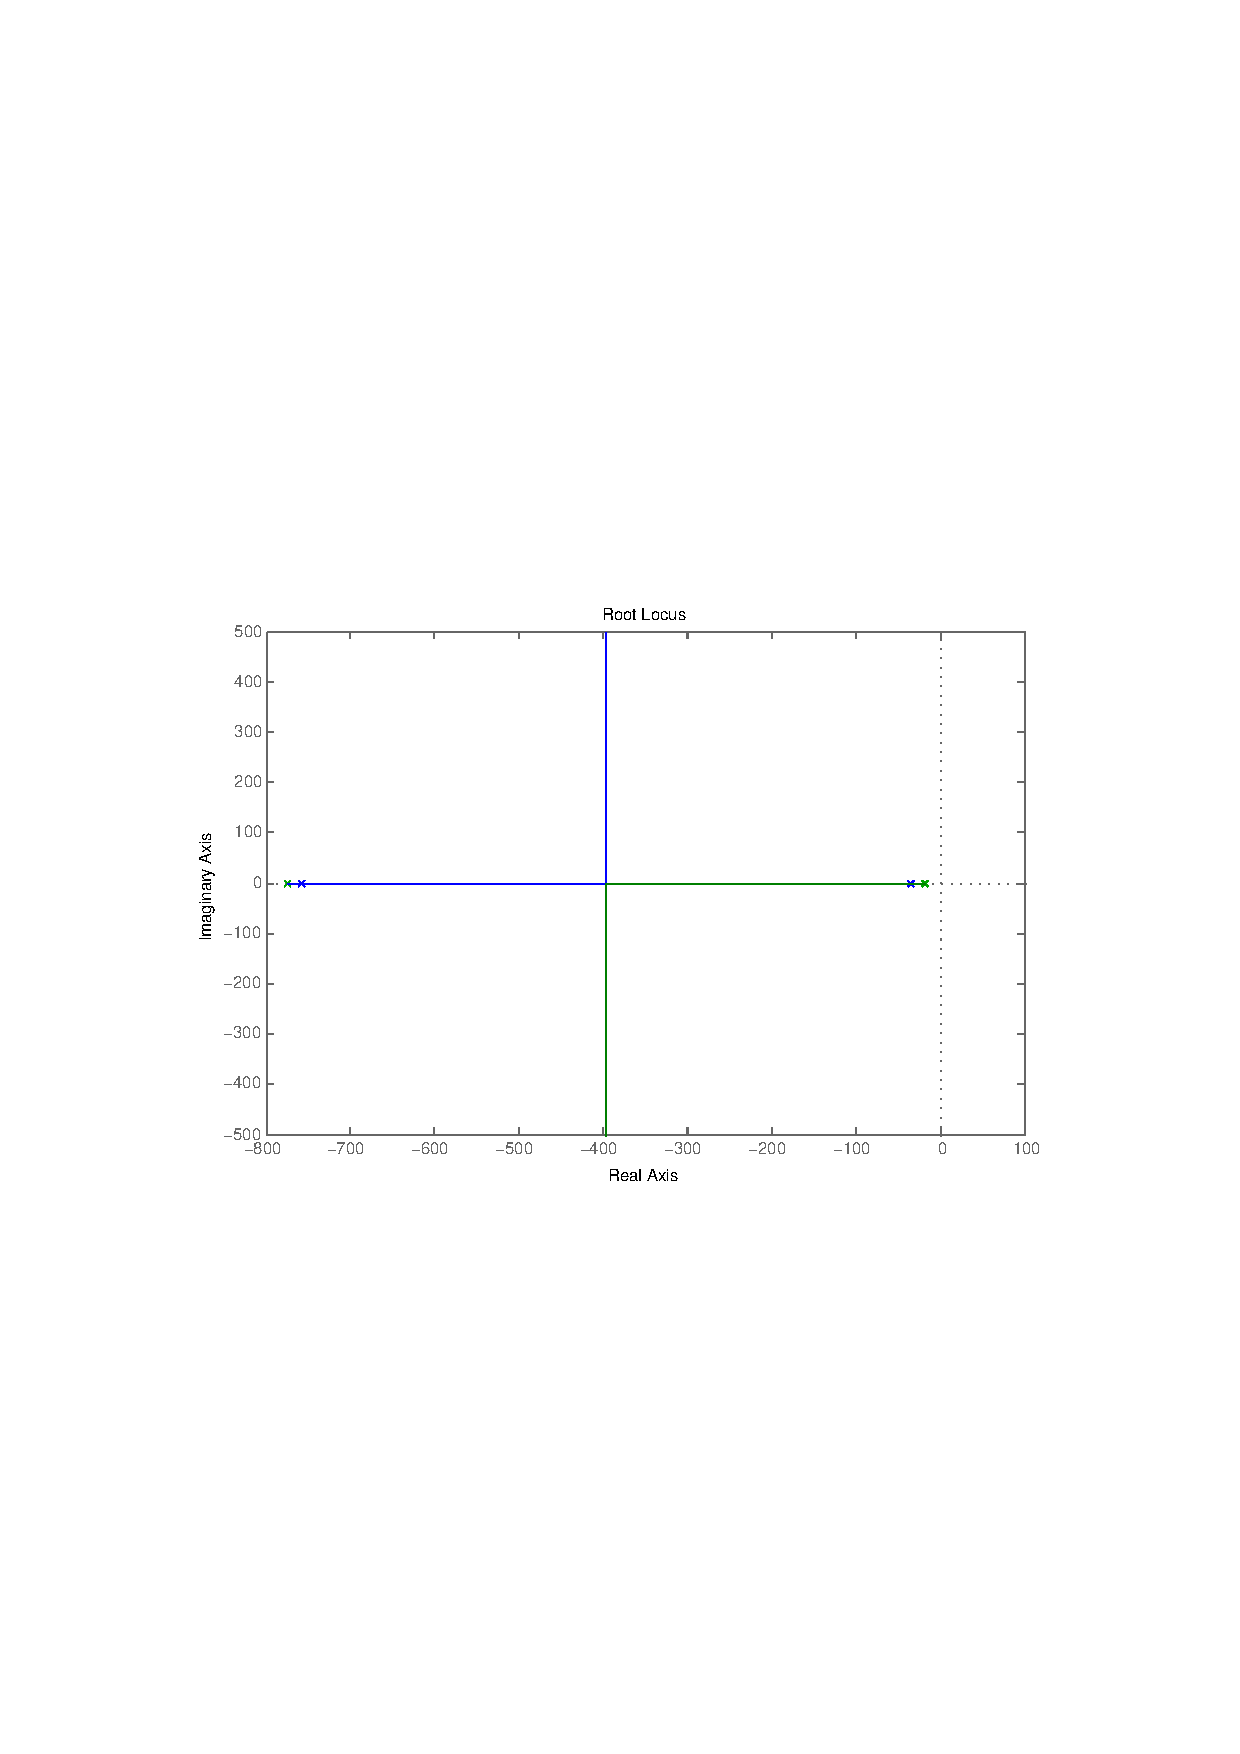
\includegraphics[width=\textwidth,trim=0 270 0 270]{graphics/rlocus_plot.pdf} %trim=l b r t (can cut off from every side)
	\caption{Shows the root locus plot the pan and tilt systems.}
	\label{fig:rlocus_plot}			
\end{figure}

The simulation is run with various parameters to find the range of values in table \ref{tab:gain_vaues}. Figure \ref{chosen_plot} shows a plot of the step response using autotuned parameters with response time 0,0175 s.

\begin{table}[htb]				
	\begin{center}
	\begin{tabular}{l|c|c|c}			
	Term & Base & Maximum & Auto tune \\			
	\hline												
P-gain pan& 6 & 450 & 145,87\\
P-gain tilt& 6 & 450 & 74,75 \\
I-gain pan& 0 & 250* & 315,36  \\
I-gain tilt& 0 & 350* & 160,79 \\
D-gain pan& 0 & 70** & 3,13 \\
D-gain tilt& 0 & 100** & 1,62\\
	\end{tabular}
	\end{center}
	\caption{Gain values derived from simulation. *@ P=30 and D=0. **@ P=30 and I=0}				
	\label{tab:gain_values}			
\end{table}

\begin{figure}[htb]
	\centering
	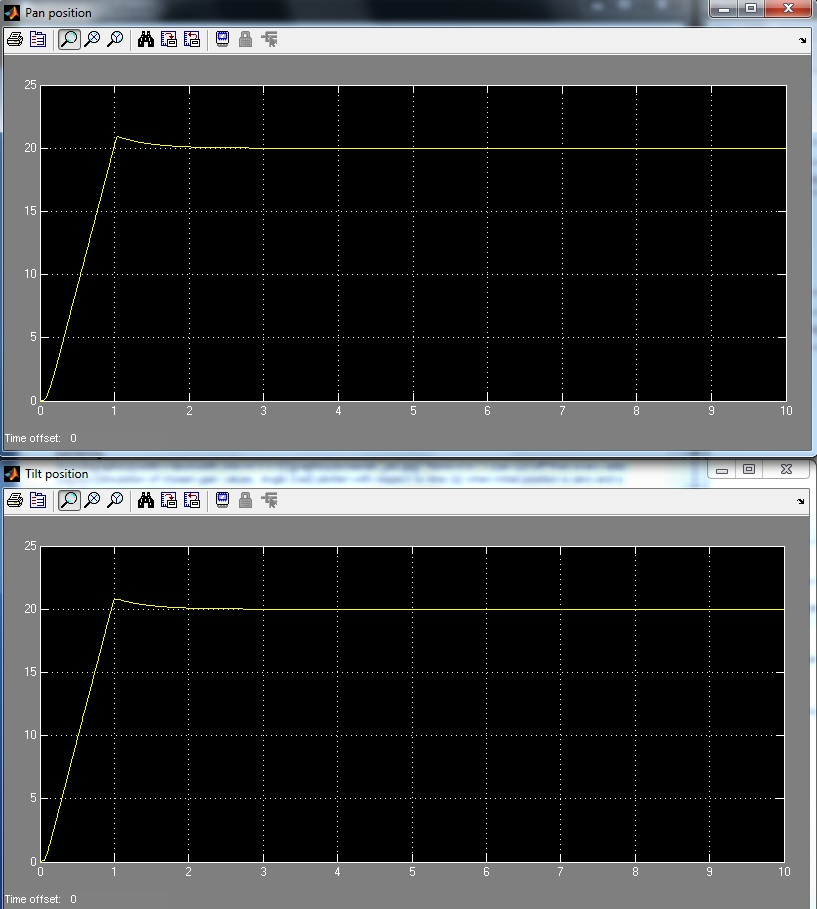
\includegraphics[width=\textwidth,trim=0 0 0 0]{graphics/screensh_pid.jpg} %trim=l b r t (can cut off from every side)
	\caption{Simulation of the autotune parameters. Angle[rad] plotted with respect to time[s] when initial position is zero and a setpoint of 20 is given as step.}
	\label{fig:chosen_plot}			% figure labels are of the form \label{fig:*}
\end{figure}

\subsection{Discussion}
The simulation of the was an easy and fast way of finding parameters for the PID regulator. Since the system has some limitations, this way of finding the range of parameters save the system from wear and tear. The autotune functionality of simulink and the ease of descretising the system also comes as credit for this approach.

In a regulator like this, there is a trade-off between having a dynamic fast responing system and having an accurate and smooth running system. In this case the objective was to obtain accuracy while remaining as dynamic system as possible.

\subsection{Conclusion}
The initial parameters for the PID regulator was found in an easy and safe way. The objective was to devolop a system able to track a position and with a steady state error of zero. Both of theese requrements were met, while keeping a faily dynamic system.

% START OF IMPLEMENTATION !!!!!!!!!!!!!!!!!!!!!!!!!!!!!!!!!!!!

\section{Implementation of PID control}
The control algorithm is implemented in the control task and all parameters are provided from the parameter server, but are cast as  floating point values for exact calculations.

When run the control task saves the value of the tick counter and when finished, it uses the FreeRTOS \texttt{vTaskDelayUntil} API to calculate when to unblock. As a starting point the control task runs at one hundred hertz frequency as verified in section \ref{subsec:control_freq}.

\begin{figure}[htb]
	\begin{center}
	\includegraphics[width=\textwidth,trim=0 0 0 0]{graphics/flowchart.pdf}
	\caption{Shows a flowchart of the implemented control algorithm}
	\label{fig:pid_flow}			
	\end{center}
\end{figure}

For calculating the error, a common format is needed. The parameter server holds the setpoint in degrees and the actual position in ticks. To be able to use some intuition about the control algorithm, degrees are chosen and the position in degrees is calculated by using a ticks to degrees factor calculated from knowing the gears and the number of ticks per motor round.
\begin{equation}
1 \ tilt \ revolution \ * 30:1 \ planet \ gear \ * 3:1 \ belt \ gear = 90 \ motor \ rounds
\end{equation}
\begin{equation}
 90 \ motor \ rounds * 12 \ ticks/round = 1080 \ ticks/tilt \ revolution
\end{equation}
This number is then used to calculate the ratio of degrees to ticks, keeping in mind that degrees have an implicit decimal:

\begin{equation}
\frac{360 \ deg \times 10}{1080 \ ticks} = 3.34\ deg/tick 
\end{equation}

The error is then calculated as the difference between setpoint and actual position and is thus a signed value in degrees.

To compare simulated values to actual values it is necessary to convert the gains so that \label{eq:conv1} and \label{eq:conv2} becomes equal. 
\begin{equation}
error \ [rad] * gain = input \ [V]
\label{eq:conv1}
\end{equation}
\begin{equation}
error \ [deg] * gain = input \ [pwm]
\label{eq:conv2}
\end{equation}

To convert from $rad$ to $deg$ the ratio is found
\begin{equation}
\frac{3600 \ deg}{2 \ \Pi \ rad} = 573 \ deg/rad
\label{eq:conv3}
\end{equation}
To convert from $[V]$ to $pwm$ the ratio is found
\begin{equation}
\frac{27.000 \ pwm}{12 \ V} = 2250 \ pwm/V
\label{eq:conv4}
\end{equation}
From equation \ref{eq:conv3} and \ref{eq:conv4} a conversion factor for the gain can be derived.
\begin{equation}
\frac{573}{2250} = 0,25
\label{eq:conv}
\end{equation}

\subsection{Implementing proportionality gain}
A first guess for the proportionality gain is to use the values provided by the autotune function in the simulation of the system. 

Since it is possible to get PWM values out of the range specified in table \ref{tab:parameters}, a maximum function is implemented, so that absolute values out of range are corrected to the maximum value.

Since PWM values below the minimum specified in table \ref{tab:parameters} does not make the motor move, a bias is added so that non-zero values are added with the bias value. This effectively narrows down the range of pwm signals to the value specified as actual pwm range in table \ref{tab:parameters}. 

A treshold is implemented so that values inside the +/- treshold area is zeroed before the bias is added. If this was not done even the smallest error would be biased.

Adjusting the P-gain is done empirically and is thus encompassed in section \ref{sec:pid_experiments_p}.

\subsection{Integrator}\label{sec:integrator}
As seen in section \ref{sec:pid_experiments_p} the system needs an integrator. Since the error grows smaller as the goal is approached, movement almost halt when approaching the goal area, making the system less accurate and slower. Therefore an integration term is implemented by adding the errror to the integration value on each run. Thereby in the situation where the error is too small to make the system move, the integration term will rise and thus add to the input. 

Normally an integration would mean the product of the value and the time since last sample, but presuming that this time is nearly constant it can be included in I-term. 

To keep the integration from going to infinity, an anti wind up filter is implemented. Wind up happens for example when the system is stopped while not at the setpoint and the integration reaches high values that has to be overcome when the system resumes.

As with the P-gain, adjusting the I-gain is done empirically and is thus encompassed in section \ref{sec:pid_experiments_i}.

\subsection{Differentiator}
By saving the error at each entry it is possible to calculate the change in the error. This term will be particularly large just after changing the setpoint, and can thus help improve the acceleration. 

The actual derivative would be the change in value over the time since last entry, but as for the integrator, this can be omitted presuming that it is constant. Since the point is to oppose the changes, the D-term of the pwm calculation is subtracted to keep the gain a positive value.

As with the P- and I-gain, adjusting the D-gain is done empirically and is thus encompassed in section \ref{sec:pid_experiments_i}


\subsection{Discussion}
The implemented PID regulator performes very well as seen from \{sec:precisionofsystem2} and the performance is almost at the theoretical limit with respect to precision. More could be done in terms of speed and setting time, but it could not be improved without knowing the explicit purpose of the system and further refinement is thus outside the scope of this project.

\subsection{Conclusion}
The decision to abandon the full state feedback regulator has been proved right, since optimal results were obtained by using a much simpler approach. Though the implemented regulator is somewhat rough, it works well and provides a base for further development.












\chapter{Low level control}\label{chap:llc}
The low level control is all implemented on a Digilent Nexys 2 test kit, featuring a spartan 3 fpga from Xilinx.
Architecturally, it is split in two nearly independent systems, one being the SPI driver and the other being the motor control.
They communicate through a shared RAM (uddyb type) block, but functions otherwise completely independant of each other.


\section{Motor interface}
The motor interface is responsible for presenting an easy to use interface to the arm processor, making it possible to control the motor torque and receive feedback in the form of pan and tilt position and velocity.
All communication is done through the RAM block as seen on figure \ref{fig:FPGAMotorArchitecture}, which means that the interface functions independently of the SPI implementation.

\subsection{Overall architecture}
The motor interface is split into two distinct parts. The PWM controller, which generates a pwm signal from a given input and a decoder controller, which reads the decoder pins, and tracks position and velocity.

A top level module is introduced to handle all memory interfacing. It houses all the individual component instances, and binds them together.

The output pins of the PWM controller A and B, is connected to the three pins of each H-bridge.
The input pins of the decoder system comes from the index pins of the hall sensors mounted on the pan/tilt system and the decoder A and B signal from the two output pins on the motors.

\begin{figure}[htb]
\centering
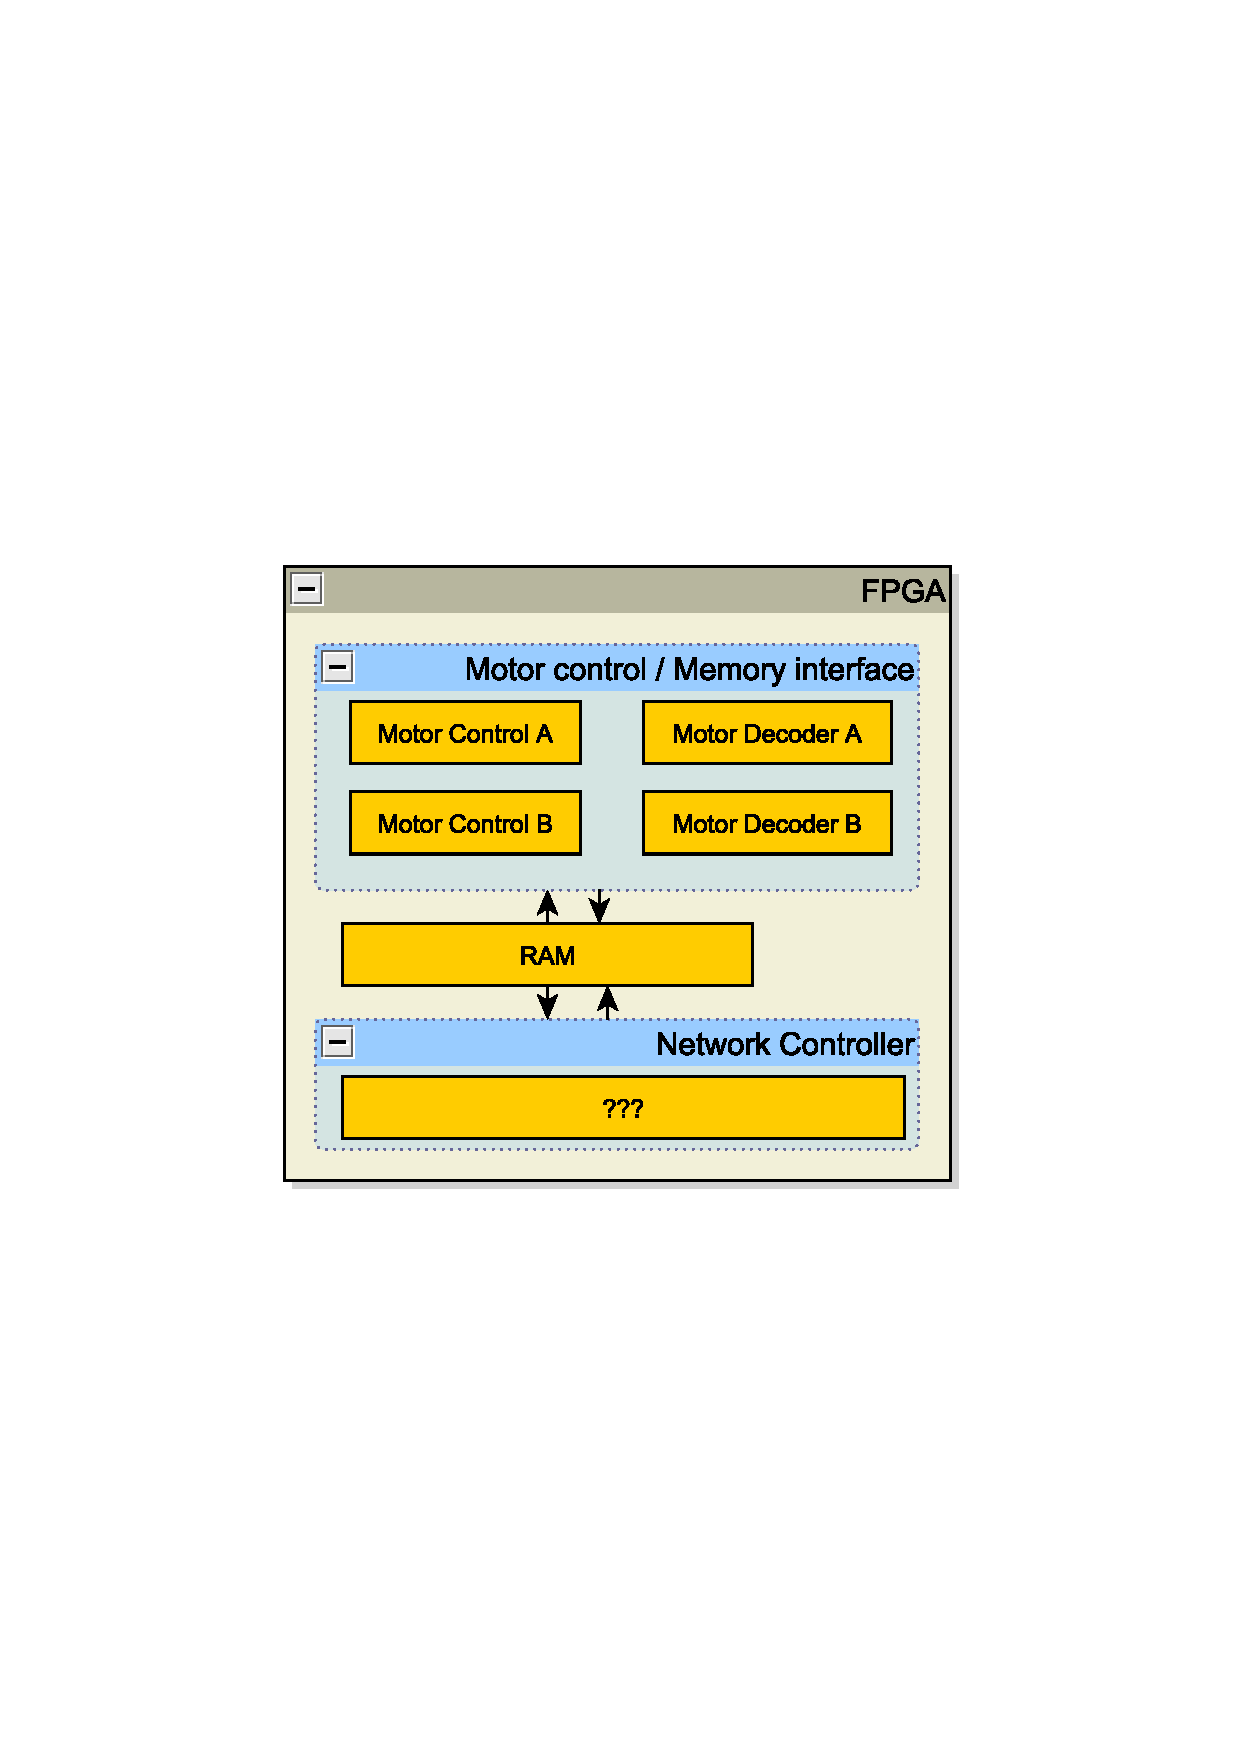
\includegraphics[scale=0.6,clip,trim=135 270 135 270]{FPGAmotorarchitecture.pdf}
\caption{FPGA architecture, from the motor interface perspective}
\label{fig:FPGAMotorArchitecture}
\end{figure}

\subsection{Memory layout}
The memory layout is as seen on table \ref{tab:Memorymapping}. The position is represented by an unsigned bit, centered around 0x8000, this is because it is easier to calculate the position without considering a sign, and it would make no difference for the control system on the arm whether the position is represented by signed or unsigned numbers.
Velocity as output and duty cycle as input is represented as a 16 bit signed twos-complement value.
This is because the sign bit makes it easy to read what the desired motor direction is.
The aux register reads position reset, and motor freerun command bits. It also sets two bits, representing whether the hall sensors indicate that the system is in zero position.



\begin{table}[htb]
\centering
\begin{tabular}{|l|r|}
\hline
Address & Value \\
\hline
0x02 & DUTY A MSB \\
0x03 & DUTY A LSB\\
0x04 & DUTY B MSB\\
0x05 & DUTY B LSB\\
0x06 & POS A MSB\\
0x07 & POS A LSB\\
0x08 & POS B MSB\\
0x09 & POS B LSB\\
0x0a & VEL A MSB\\
0x0b & VEL A LSB\\
0x0c & VEL A MSB\\
0x0d & VEL A LSB\\
0x0e & AUX FROM ARM\\
0x0f & AUX TO ARM\\
\hline 
\end{tabular}
\caption{Memory locations of control registers}
\label{tab:Memorymapping}
\end{table}


\section{Motor control block}


The motor control block is split into 3 seperate modules.
The PWM generator, the signed-to-magnitude splitter, and the Motor AUX control as seen on figure \ref{fig:pwmblock}.
It takes a 16 bit signed integer and a control bit as input, indicating whether the motor should be driven by a pwm signal, or if it should be set in free run mode. 
When the motor is not in free run, the enable pin on the H-bridge is high, and the pwm signal changes between the braking and running state. If the free run bit is set, the H-bridge is disabled and no pwm signal is generated.

\begin{figure}[htb]
\centering
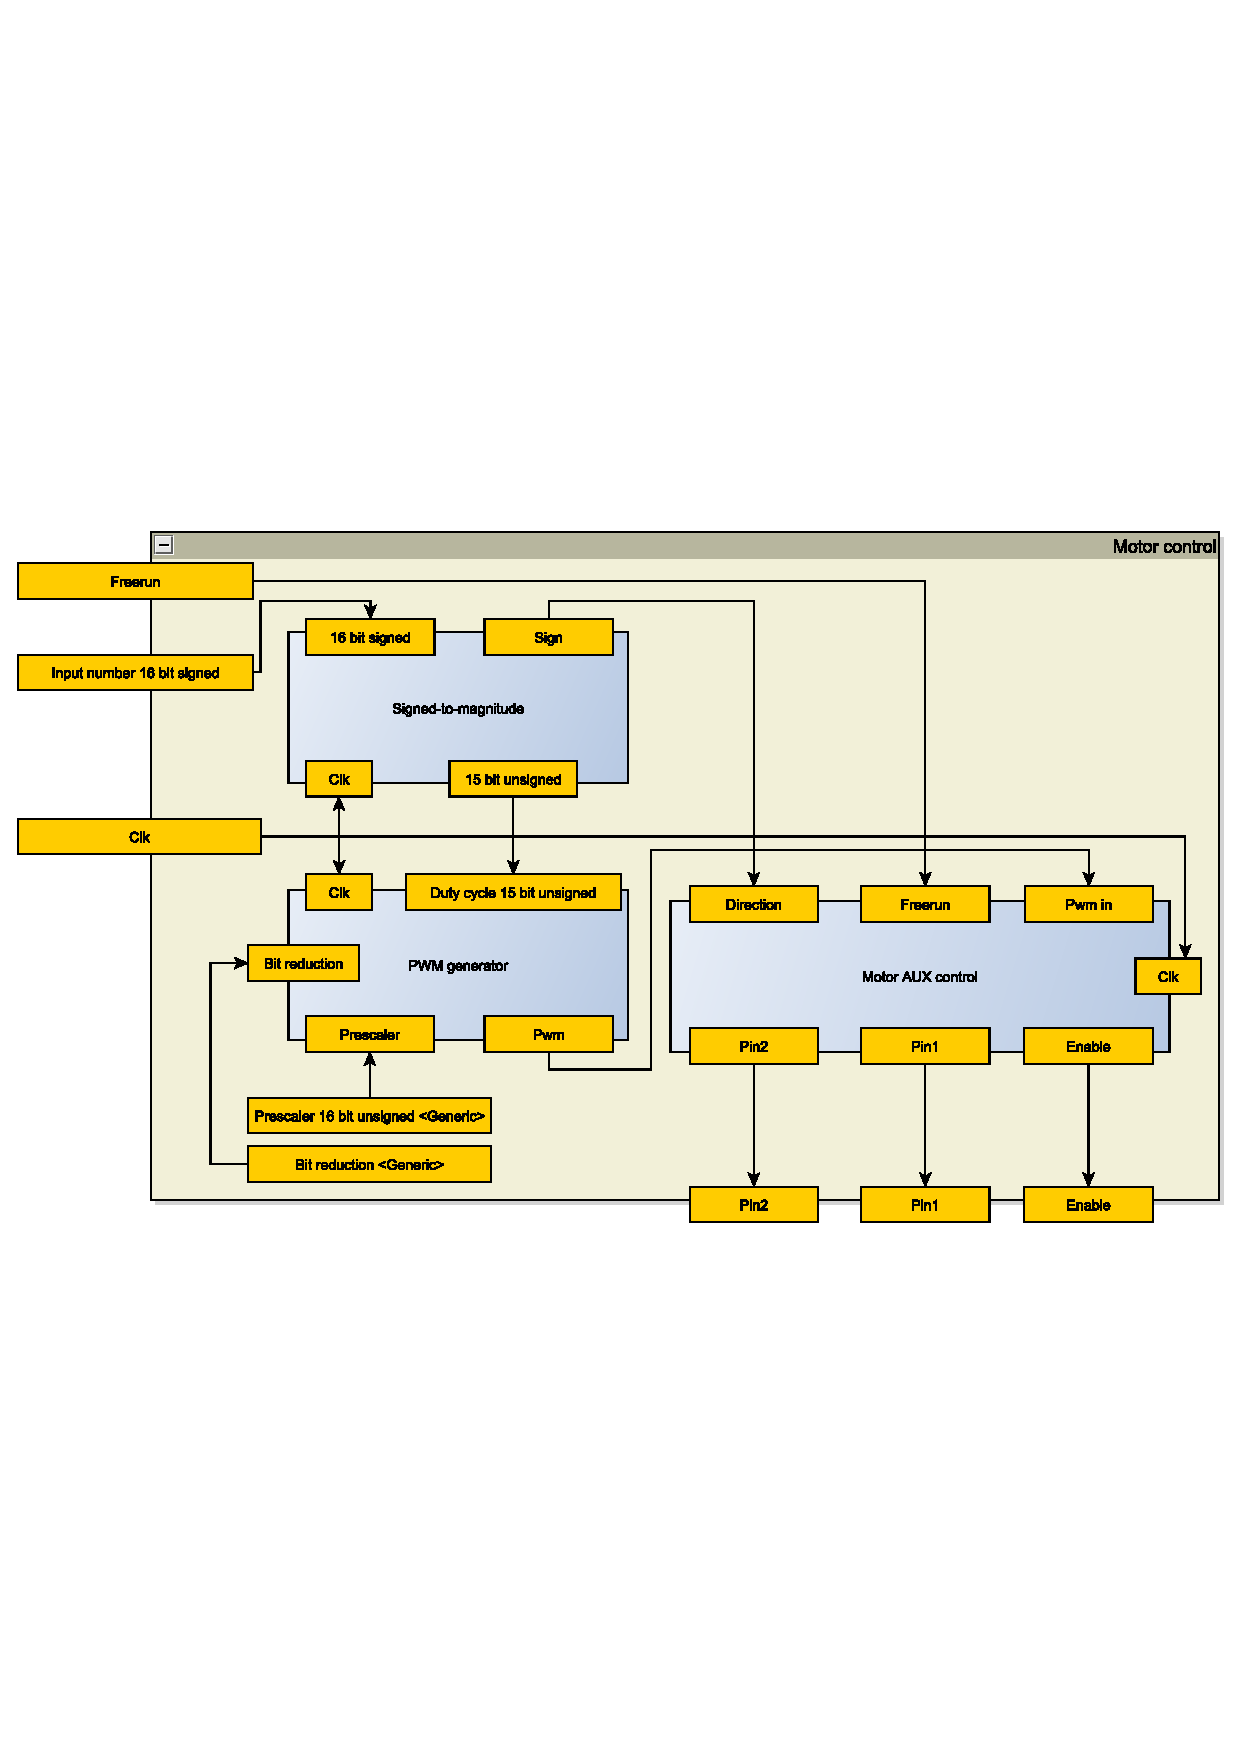
\includegraphics[width=\textwidth,clip,trim=0 250 0 250]{PWMblock.pdf}
\caption{Block/signal layout of the Motor control block}
\label{fig:pwmblock}
\end{figure}

\subsection{PWM generator}
The PWM generator takes a clk signal and a duty cycle (15 bit unsigned value) as input. It also takes two generic parameters as input. A prescaler value to decrease the frequency, and a bit reduction parameter to increase it. These allows the PWM block to be configured for a desired frequency.

Internally the pwm generator consists of a counter register that is decremented each tick as seen of figure \ref{fig:pwmchart}. If the counter is less than the input, the output is 1 otherwise it is zero.
If the counter value underflows, it is set to the second highest value it can represent. This ensure that the PWM block is able to output high and low value dc if needed, at the cost of lacking an extra bit of resolution.

The bit reduction parameter effectively reduces the amount of significant bits in the counter and value signals.
The prescaler is used to introduce a delay between each tick.

The frequency of the PWM needs to be at around 20khz or above. If it is lower than that it is in the audible range of frequencies which would be an annoyance. If the frequency is too high, to much energy is lost in the transistors, not to mention the fact that an h-bridge has a switching time, which would distort the actual duty cycle output.

For calculating the pwm frequency the following formula is used: 
\begin{equation}
F_{pwm} = \frac{F_{xtal}}{2^{number of bits}}
\end{equation}

Without using prescaler and bit reduction values, the pwm frequency is calculated with 16 bit resolution and a 50 mhz internal clock, which gives a resulting frequency:
\begin{equation}
\frac{50 mhz}{2^{15}} = 1525.88 hz
\end{equation}

This is way to low, and therefore the amount of used bits are reduced by four giving the frequency:
\begin{equation}
\frac{50 mhz}{2^{11}} = 24414.1 hz
\end{equation}
Which is just above the minimum frequency requirement.

\begin{figure}[htb]
\centering
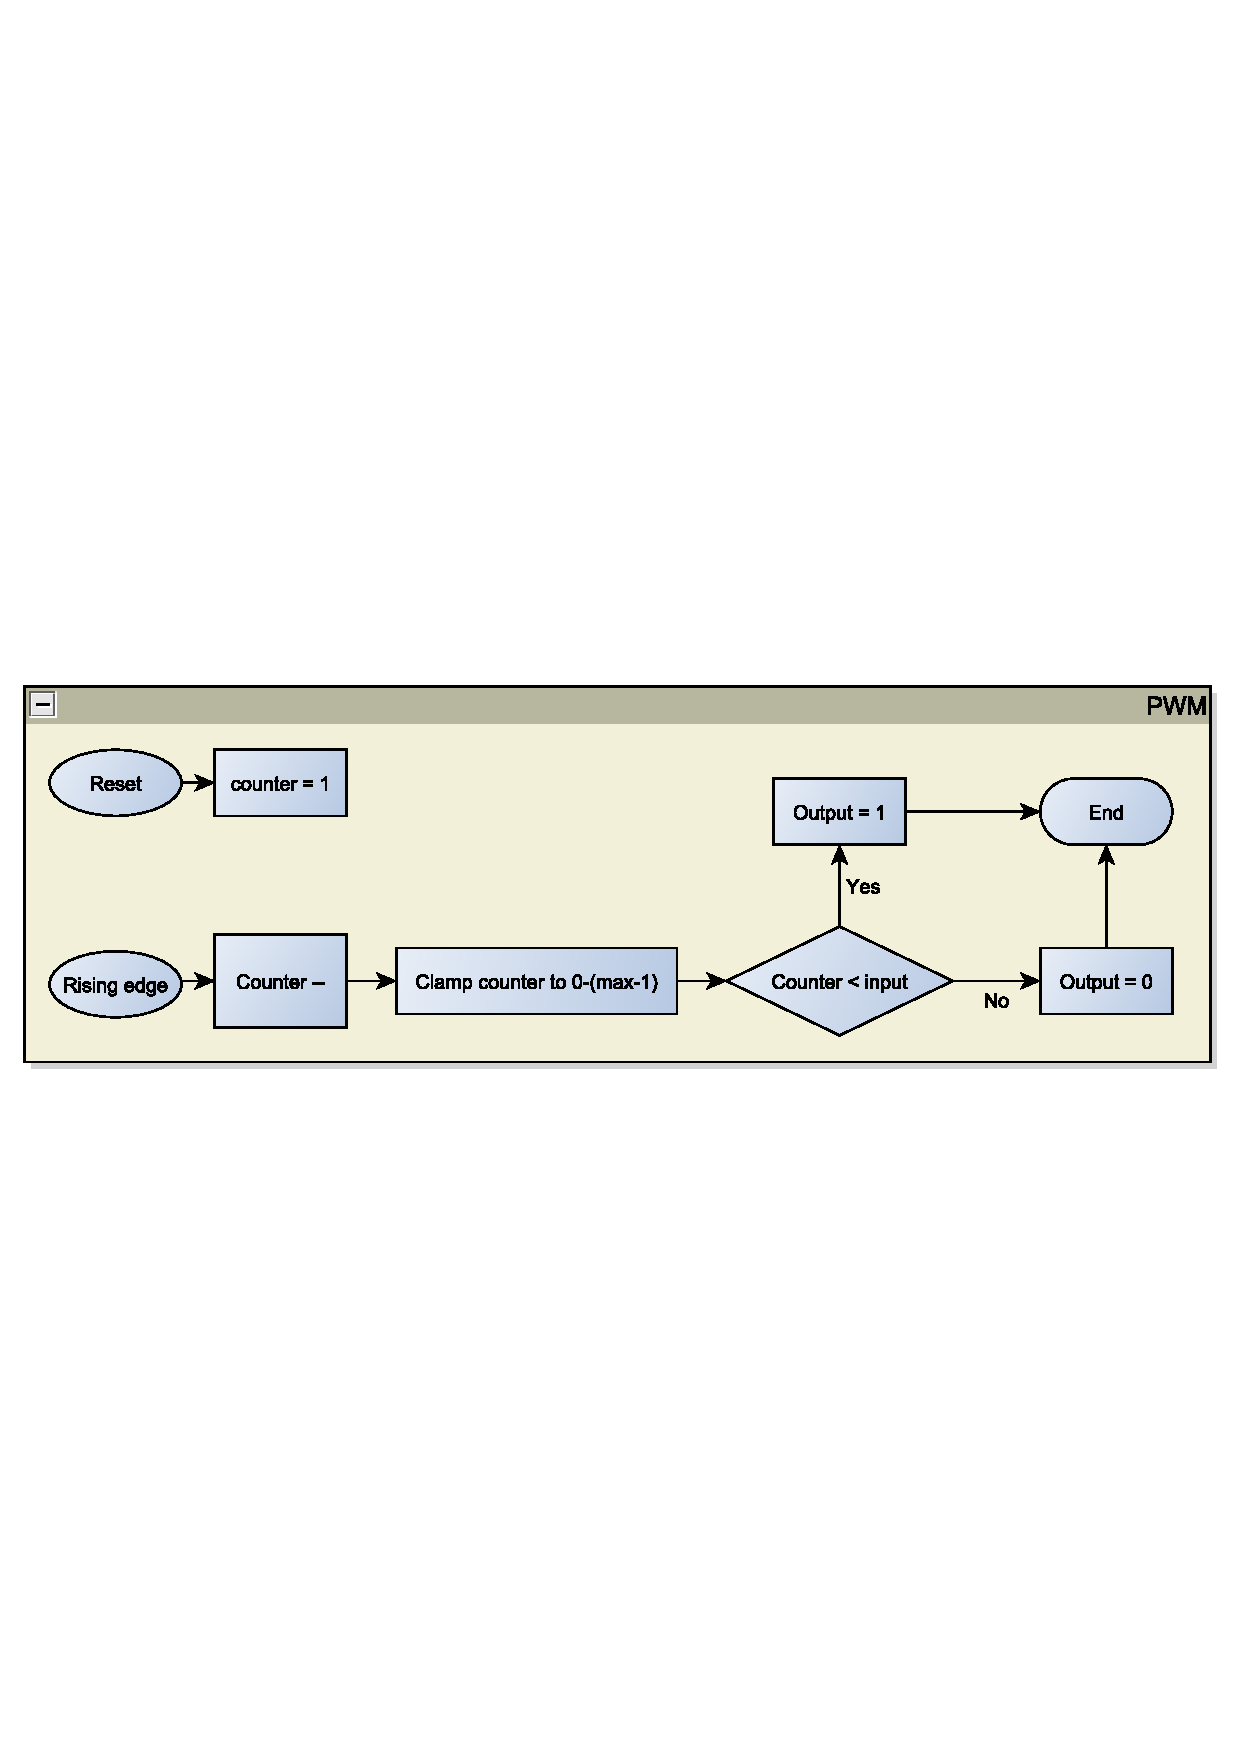
\includegraphics[scale=0.6,clip,trim=10 330 10 330]{PWMexecution.pdf}
\caption{Flowchart of the pwm generator}
\label{fig:pwmchart}
\end{figure}

\subsection{Signed-to-magnitude splitter}
The signed-to-magnitude splitter takes a signed 16 bit integer as input and outputs the sign and magnitude separately.
The magnitude is computed as follows:
If it positive, its just the 15 last bits, if it is negative the twos compliment value is the output.

\subsection{AUX control}
The aux control takes the direction, pwm and freerun signals as input, and output the pwm signal on either pin 1 or 2 of the h-bridge. If the freerun pin is not high, the enable pin is high, if the freerun pin is high, no pwm is output, and the enable pin is low.

\section{Decoder system}
The decoder system is responsible for reading the state of the pan/tilt system from the hall sensors mounted on the system, and the quadrature encoders on the motors. 
It outputs a relative position from the reset point and a velocity for each of the two axes, as precise as possible.

The decoder is split into 4 major components: The Input filtering, the quadrature decoder, position normalizer and velocity estimator components, as seen on figure \ref{fig:decoderblock}. 



\begin{figure}[htb]
\centering
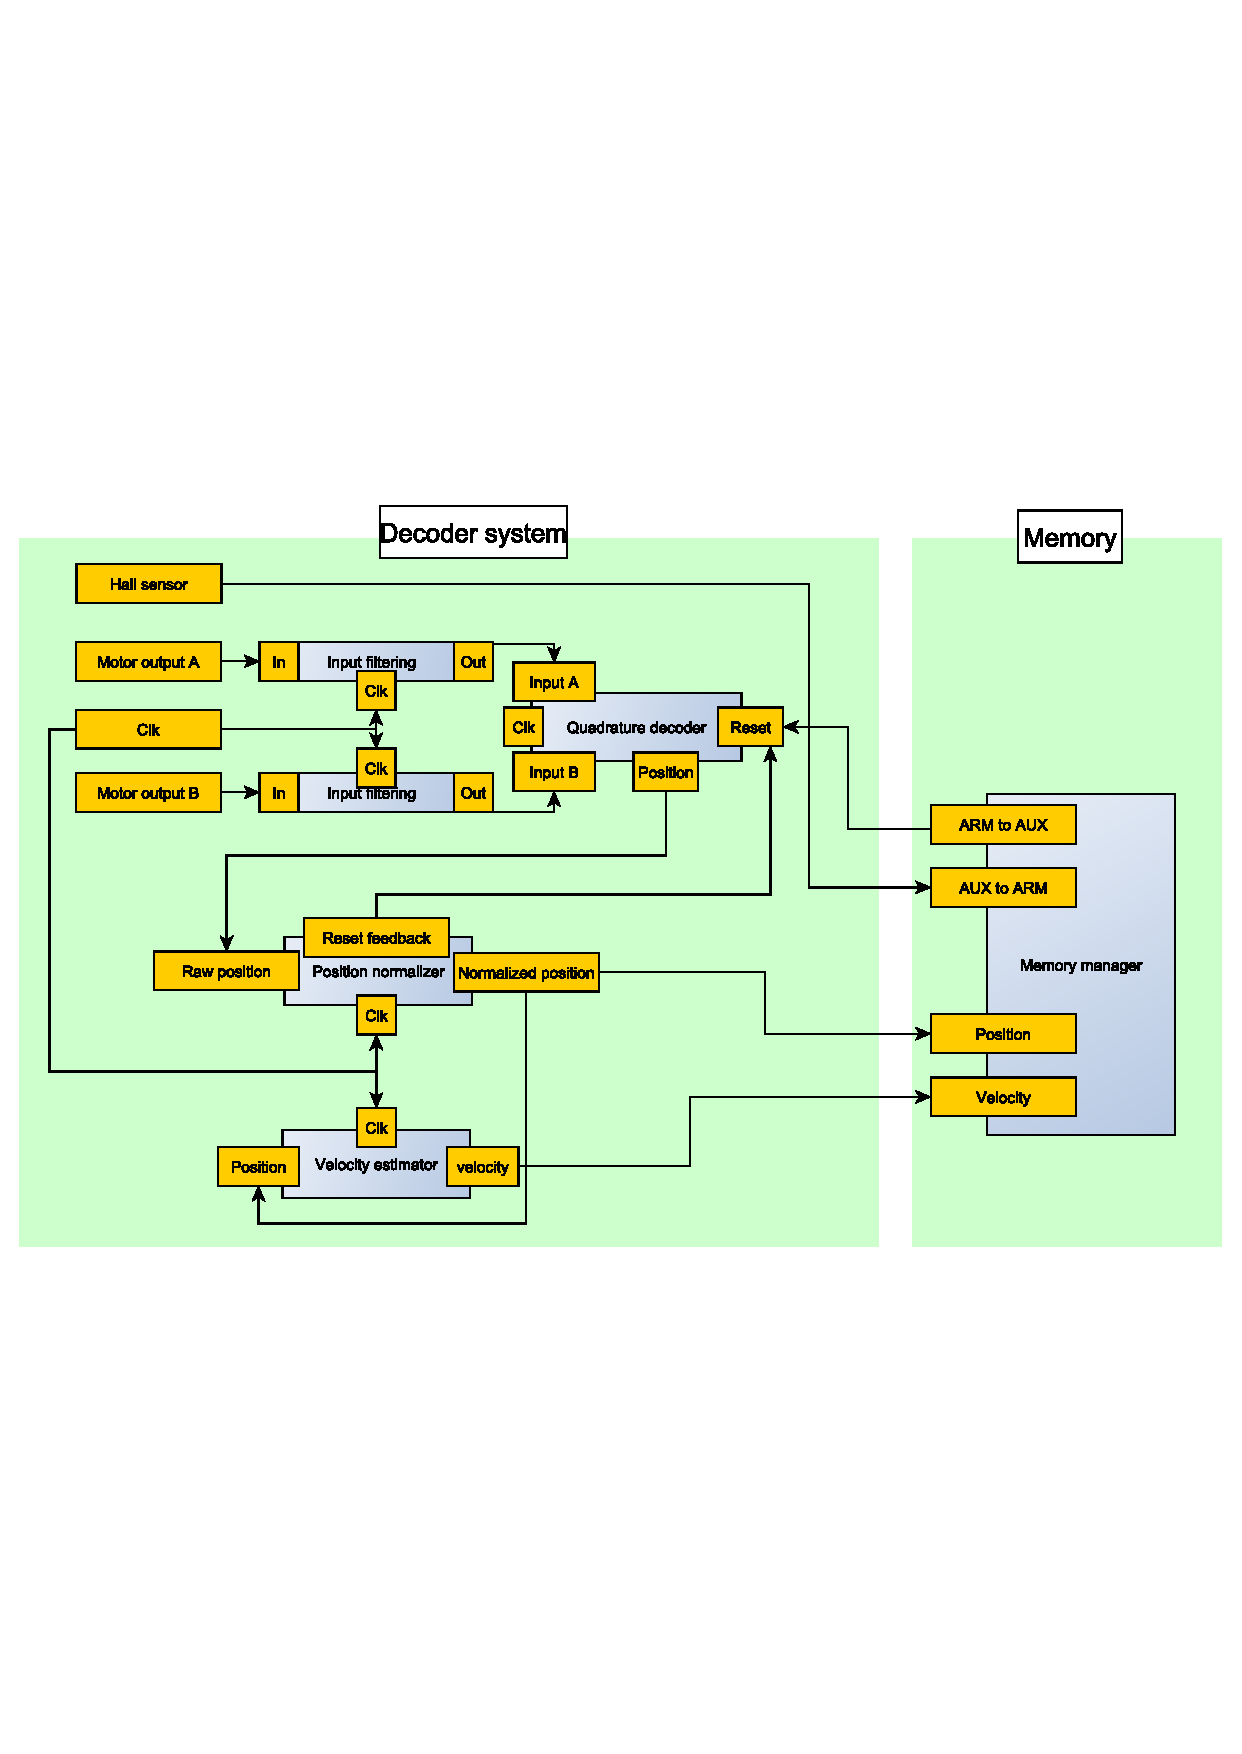
\includegraphics[width=\textwidth,clip,trim=2 250 2 230]{decoderblock.pdf}
\caption{Block/signal layout of the decoder system}
\label{fig:decoderblock}
\end{figure}


\subsection{Input filtering}
Since the input signal comes from the outside \"real\" world, unwanted noise must be removed for it to be used. However, the regulator depends on this signal, so care must be taken not to introduce an unwanted large delay, as that would make the signal  useless.

To remove noise, a simple de-bounce, with hysteresis is applied, it features a counter that, for every clock pulse counts up if the input signal is high and down if it is low.
When ever the counter rises above a threshold, and the filter is outputting a low signal, it changes to high. The same opposite when counting down.
The counter part of the process introduces a delay in output changes, so that a lot of switching back and forth between high and low, will not affect the output. The hysteresis helps negate short burst errors in the input. 

The distance between the lowest value possible in the hysteresis counter, and the value that causes a switch to high the in output,

The difference between the hysteresis counters lowest value and the rising edge value, or the highest value and the falling edge value, whichever is highest, determines the maximum frequency the input filter will let through, as well as the delay introduced in the position counter.

A set of values must be chosen that filters the signal adequately, without producing error signals. The tilt rotor has been observed to have approximately 1000 ticks pr. full revolution, and with full power to the motors, max one rotation pr. second.
This means that the input filter should be able to let a 1khz signal through at least. \\ 
Since external forces can temporarily push the system to higher frequencies, it is assumed that a max frequency of 1mHz should cover all but the most extreme cases.

This means that the maximum input delay can be 50 clock ticks.
In this assignment, a set of values was then chosen within the constraints: 
Lowest value: 0
Maximum value: 20
Low hysteresis: 4
High hysteresis: 16

These values give a maximum input delay of 16 clock ticks(320 ns) which is sufficient for this application.

\subsection{Quadrature encoder}
The quadrature encoders job is to convert the two decoded signals from the motor, to a relative position. The signal is generated from two hall sensors that are positioned 90 degrees apart. Giving 4 different output states, each state indicating what quadrant the motor is positioned in, an example of the signal can be seen in figure \ref{fig:decodersignal}.
\begin{figure}[htb]
\centering
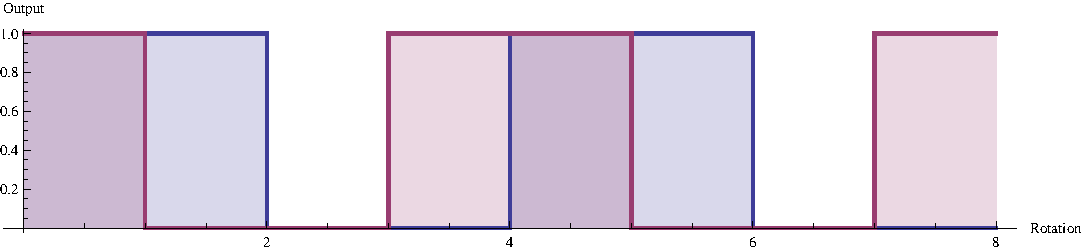
\includegraphics[width=0.9\textwidth,clip,trim=0 0 0 0]{ddecodersignal.pdf}
\caption{Example decoder output from a motor with constant speed}
\label{fig:decodersignal}
\end{figure}
The decoding process can be thought of as a state machine (with the encoder output being the state variable), where a state transition corresponds to a movement step in one of two directions.
When the decoder is first powered, a default position value is kept, and then incremented or decremented according to the statetransition. The default value is set at 0x8000 unsigned integer, as this allows for the maximal displacement in either direction. 
Overflow is not handled in this module, as it is not its job to know anything about the configuration the motor is in, however an external reset pin is provided, which returns the counter to 0x8000. (This reset signal is incidentally powered by the position normalizer module).
The situation where the input pins both change in one clock cycle is not handled by the system.

\begin{figure}[htb]
\centering
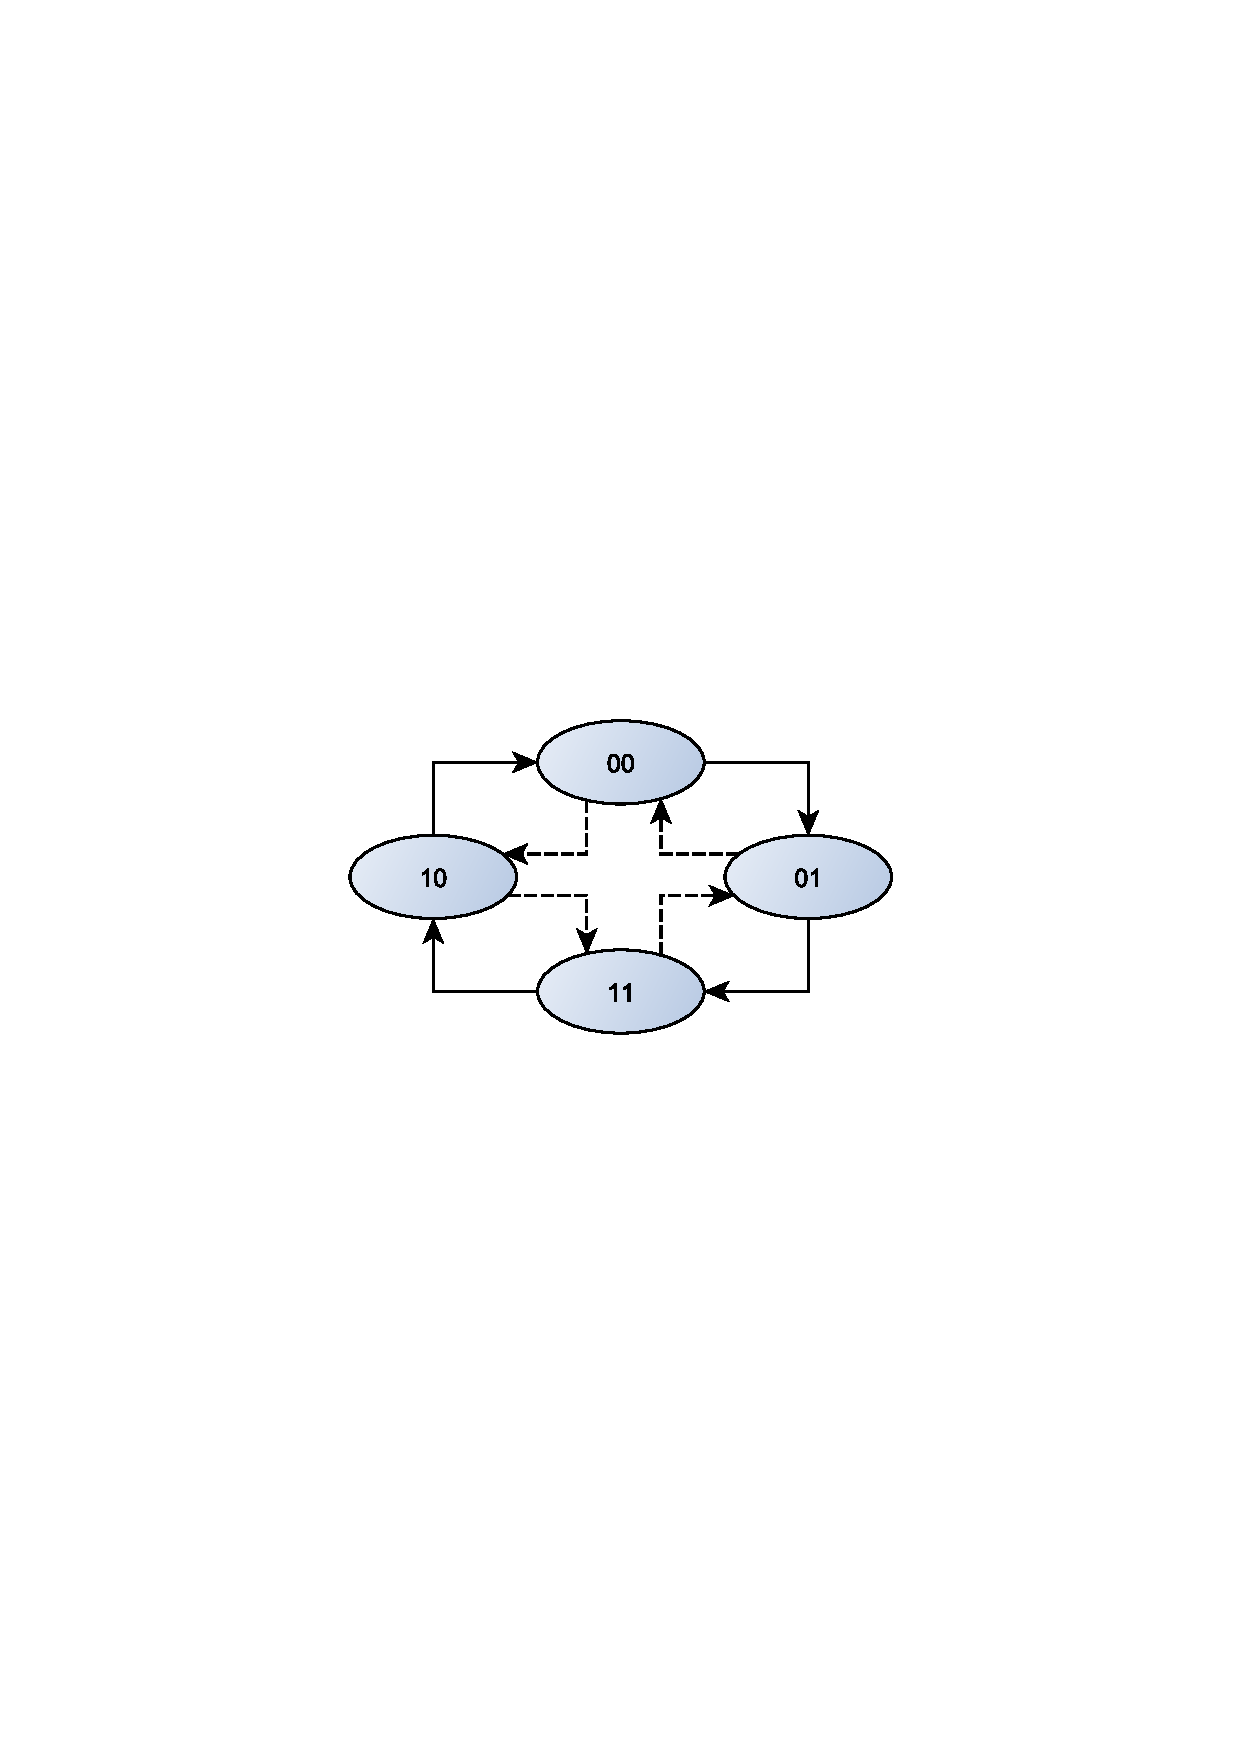
\includegraphics[scale=0.6,clip,trim=130 330 130 330]{decoderstates.pdf}
\caption{State diagram of the decoder module, the stipled arrows indicate a negative clockwise, the solid indicate a counter-clockwise or vice verca.}
\label{fig:decoderstate}
\end{figure}

\subsection{Position normalizer}
The position normalizer block is used for any conversions/adaptations of the raw position value necessary. For instance the position could be converted to radians or similar. It also features a feedback reset signal, if this should be necessary. 
In the final version of the application, this block does nothing other than let the input go directly to the output.
Should any automatic reset system be required, based on the position, this is the block to handle it.

\subsection{Velocity estimator}
The velocity estimator is responsible for measuring the velocity based on the counter input.
There are several methods available for measuring the velocity, each with its drawbacks and strengths.
A simple method is to compare the position with a fixed frequency, so that for instance each second, the velocity is the difference between the position before and after a second has passed. This has the advantage of being easy to implement and test, also everything is implemented with integers. The drawback is that this method can produce wildly varying velocity measurements, especially if the actual velocity produces a position change frequency just above or below the sampling frequency.
This drawback can be offset by \"tuning\" the sampling frequency until a desirable behavior has been reached.
Another method is the secant method, where the time between each change of the position is measured. The reciprocal of this is then the velocity. The advantage of this method is that it is, in theory, very precise. The drawback is that a floating/fixed point division is necessary, in order to obtain the correct result. Also should there be any imprecision in the motor decoding, it will be reflected strongly in the measured velocity. Furthermore, a time-out period must be included, for there is no edge to detect when the motors stop moving.

In both cases smoothing of the result can be needed. By using a running average filter, the velocity measurement can be smoothed over many samples, but a first order delay in the measurement is introduced.

In the final application, there is no velocity estimator, since it is not needed in the chosen regulation method, however the two mentioned measurement methods are included in the codebase for completeness sake.


\section{Watchdog}
Since all control commands are buffered in the ram until updated again, the fpga has no way of knowing if the SPI link has been lost, either because of the ARM processor crashing, or cable failure etc. This means that in case the case of the link being lost, it will continue going if any velocity command has been issued before the connection died. To correct this problem, a watchdog is implemented. It outputs an enable signal as long as there is a link between the fpga and ARM. 
To detect the link presence, two registers in the control register are constantly incremented, and the watchdog keeps a watch on them, should they fail to change within a set time, the watchdog will stop all motor activity.
The watchdog module is not included in the final application due to time constraints.




























\chapter{Communication protocol}\label{chap:comm}
For the main hardware components to be able to communicate, some kind of network communication has to be defined. Throughout this chapter the communication hardware, methods and final design of this network will be introduced.

\nomenclature{SPI}{Serial Peripheral Interface}

\section{Low level protocol specification}
In \marginnote{Not sure about the exact placement of each part of section. Let's talk about that some day!}[-25pt] the assignment proposal it is given that the communication interface between the FPGA and LM3S6965 microcontroller must be SPI. There are no formal SPI protocol standards however, so it must be decided how the link will work. The Stellaris SSI\footnote{Synchronous Serial Interface} module supports three different interfaces: Freescale SPI, MICROWIRE and Texas Instruments SSI. The main difference between these three formats is how they handle each individual serial frame.

The Freescale SPI mode of operation is chosen, as it enables full-duplex transmission (which MICROWIRE does not) and because of the way the select signal (\texttt{SSIFss}) works in this mode. Using the Freescale frame format, the \texttt{SSIFss} is high while the communication line is idle. \marginnote{This calls for an illustration} It is then pulled low while sending a frame. Pulling it low thus signifies the beginning of a frame, and pulling it high tells the slave that the frame is at its end. The Texas Instruments SSI format works by instead pulsing its \texttt{SSIFss} signal for only one \texttt{SSIClk} period to signify the beginning and ending of a frame. This is deemed more error prone as there is no time in-between frames to synchronize. Freescale SPI has one \texttt{SSIClk} period in-between frames, where \texttt{SSIFss} gets pulled high, allowing the slave a chance to "catch up".\nomenclature{SSI}{Synchronous Serial Interface}

The LM3S6965 microcontroller will be operating as master and the FPGA as slave, letting the microcontroller when communication should take place.

%------------------------------------------
\section{SPI introduction}
SPI is short for Serial Peripheral Interface, and is a commonly used standard for internal communication between hardware. Because SPI is a commonly used transmission interface, this will only contain a short introduction. The \marginnote{Check me}{simplest} SPI connection consists of a master, a slave and 4 signal lines: A clock, a signal from master to slave (MOSI\footnote{Master Out Slave In}), a signal from slave to master (MISO\footnote{Master In Slave Out}) and a slave select (SS) signal. The clock is used to control when to put data on the signal lines, and is always controlled by the master device. This way the master device always controls when there is data available on the signal lines, and at what data rate the it is send. An effect of this is that, for the master to be able to get a reply from the slave, some extra data needs to be send to activate the data carrying clock. The synchronisation between the clock and the data on the MOSI and MISO lines can be set up in four different ways, depending on the clock phase (CPHA) and polarity (CPOL). The slave select signal is used to enable the transmission on the slave device. When pulled low, the slave device starts listening for data from the master device. This enables the use of the clock, MOSI and MISO lines for multiple devices. 
% What is SPI
% Limitations

%CPOL CPHA

% SPI stands for Serial Peripheral Interface
% Used for moving data simply and quickly from one device to another
% Serial Interface
% Synchronous
% Master-Slave
% Data Exchange
% Data on SCK  (the clock rate can vary, unlike RS-232 style communications)
% SPI sync modes
% WIKI fact:  frequencies are commonly in the range of 1�70 MHz

%\subsection{Hardware support}
% Support on ARM development board -- The LM3S6965 controller includes one SSI module that provides the functionality for synchronous
% serial communications with peripheral devices, and can be configured to use the Freescale SPI,
% MICROWIRE, or TI synchronous serial interface frame formats. The size of the data frame is also
% configurable, and can be set between 4 and 16 bits, inclusive.

% Separate transmit and receive FIFOs, 16 bits wide, 8 locations deep

%\subsection{Inspiration for protocol}
% ArcNet / PA10
% CAN / DeviceNet
% ADNS9500 Mouse sensor, IMU sensor
% - What is it used for, and why is it interesting to look at?
%The first approach for designing the SPI protocol was to look for  
\section{Protocol requirements}
Selection the right protocol design for a project greatly depends on the requirements from the other parts as the system. Such requirements would include: 
\begin{itemize}
\item Noise on transmission lines (Need for error correction or detection)
\item Security (encryption)
\item Package synchronisation (Start and stop flags)
\item The size of data to be transmitted (Minimum transmission speed)
\item Timing criteria (Do we need to know how old the data are)
\end{itemize}

Because the data only needs to travel a short distance, noise and security is not considered as a problem in this project. Even if noise should occur, a lot of things could be done to the physical parts to solve this without involving redesign of the protocol (Ex. paired and shielded cables). 
The protocol are using SPI, so there is no need for synchronising the packages, as this can be done by the SS signal line. This eliminates the needs for overhead such as start or stop flags on packages. 
\marginnote{Read and comment if it's good enough}The ARM runs the SPI connection at a speed of 1MHz. Each clock pulse transmits 1bit, so 1MHz will carry 1Mbps = 128KBps. With this transmission rate, it will be possible to read or write an entire 32byte memory block at a rate of $\frac{128KBps}{32B} \approx 4KHz$. The ARM is capable of running the SPI at much greater speeds then 1MHz, and a update rate of 4KHz is a lot more then needed, considered physical speed limitations of the \marginnote{pan/tilt}{pan/tilt} system.


\section{Protocol ideas}
\label{spi_protocol_ideas}
During the design of the protocol three approaches were considered. These three approaches and the final protocol solution are described below.


\subsection{Specialised protocol}
The first approach was to design the protocol to carry just the information that needs to be exchanged between the FPGA and ARM boards. A data package would then consist of a header followed by a series of only the needed data. This idea had the advantage of a low overhead on the protocol and thereby a minimal need for resources on the platforms. This idea was discarded, because a change in the data requirements would require a redesign of the protocol.

\subsection{Memory synchronisation protocol}
Another approach to the protocol design was to make a protocol to synchronise a static sized memory between the two platforms. The idea was to take advantage of the 16bit x 8 FIFO on the ARM platform, so one package would fit exactly into it. The advantage would be that the ARM processor only needs to be interrupted when the FIFO was full. A similar solution would then be written in hardware to the FPGA, making this solution quite efficient. The large amount of data in one package would allow a CRC or checksum to be implemented without too much overhead. An example of how this protocol could be made is shown in figure \ref{fig:spi_protocol_format_memsync}.

\begin{figure}[htb]
	\begin{center}
	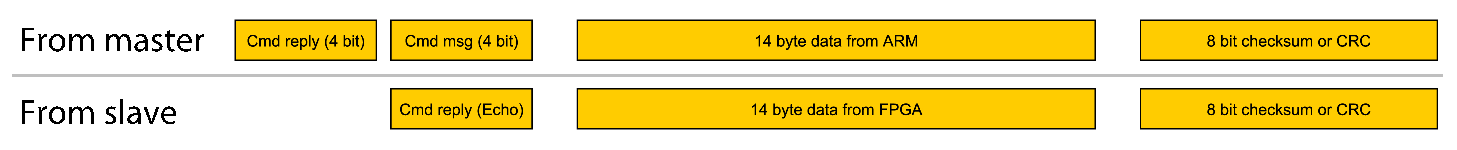
\includegraphics[scale=0.6,trim=20 0 0 0]{graphics/spi_protocol_format_memsync.pdf} %trim=l b r t (can cut off from every side)
	\caption{An example of the protocol design with the memory synchronisation protocol approach}
	\label{fig:spi_protocol_format_memsync}			% figure labels are of the form \label{fig:*}
	\end{center}
\end{figure}

The first four bits from the master decides what the slave shall respond. The next four bits describes what the master is sending to the slave. After the slave has received the first four bits, it immediately echoes the command followed by the requested data.

\subsection{Generic protocol}
\label{spi_generic_protocol}
The generic approach was to make the protocol compatible with the protocol of other SPI devices. Because a lot of SPI devices uses specialised protocols, there is not a generic approach as such. Some devices tough share a way of reading and writing registers on the hardware, which in this document will be referred as a generic way. Using this protocol will give the great advantage of both reusable code/hardware, fairly easy implementation and good scalability. The generic design approach was chosen as most appropriate solution for this project and will be described in greater details in section \ref{spi_rotocol_design}.


%\section{Protocol selection discussion}
%Something that sounds smart or REMOVE ME.

%The ADNS9500 mouse sensor and ADIS16405 IMU sensor SPI interface protocols were used as reference designs, as these are well known form earlier projects.  

% Burst mode
% i2c
% error correction / detection
% Error detection
% Room for extending protocol

\section{Protocol design}
\label{spi_rotocol_design}
It has been decided to use a generic\footnote{See \ref{spi_generic_protocol} for a definition of generic} way of communicating with SPI between the FPGA and ARM board. Other ideas were considered and can be read about in \ref{spi_protocol_ideas}.
The main advantage for choosing a generic design is the simple implementation and compatibility with other SPI devices. The ADNS9500~\cite{SPI_ADNS} mouse sensor and the ADIS16405~\cite{SPI_ADIS} IMU sensor were used as protocol reference devices, as these has been used in previous projects. The main difference between the protocol in these two devices are the length of the carried data. The ADNS9500 reads and writes only 8 bits at a time, where ADIS16405 supports 16bit data sizes. The 8 bit solution was chosen as reference.

For synchronisation of clock and data on the signal lines, mode 0 was chosen. Mode 0 is when data is available on clock rising edge and changes on falling edge.

% Depending on the address it can be read only, write only or read/write. 
The general idea is that the SPI slave has a memory block, which the SPI master can read and write from. The list of addresses are determined by the hardware modules on the FGPA and can be found in table \ref{tab:Memorymapping}. The protocol itself is pretty straight forward. The MSB determines if it is a read or write operation, and the last 5 bits determines the address or function. The two bits in between are reserved for future use, and should always be set to zero. The five address bits in the current design gives access to 32 bytes of memory on the slave device, which is enough to hold the data for this project. The command structure is shown in figure \ref{fig:spi_protocol_cmd_structure}. Both reference devices supports a burst command, where a series of relevant data are sent as response of a single command. There was no need to implement such functionality in this design. How the reading and writing is done is described below.
\begin{figure}[htb]
	\begin{center}
	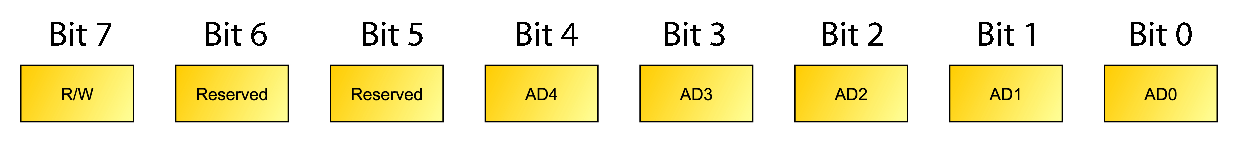
\includegraphics[scale=0.65,trim=0 0 0 0]{graphics/spi_protocol_cmd_structure.pdf} %trim=l b r t (can cut off from every side)
	\caption{Bit structure of the SPI command send from master to slave}
	\label{fig:spi_protocol_cmd_structure}			% figure labels are of the form \label{fig:*}
	\end{center}
\end{figure}


\subsection{Reading from slave device}
When the master needs to read from the slave device it sends a byte with the MSB\footnote{Most significant bit} to low, and the last five bits according to the address to be read. Meanwhile the command is send, the slave may be sending the response from last command, or just zeroes if it has nothing to return. For the master to be able to receive the response, it needs to send a byte because SPI is synchronous. This may be the next command or just zeroes. The reason for this is, that the communication is always initiated from the master device on SPI. A read command sequence is shown in figure \ref{fig:spi_protocol_command_structure_read} 

\begin{figure}[htb]
	\centering
	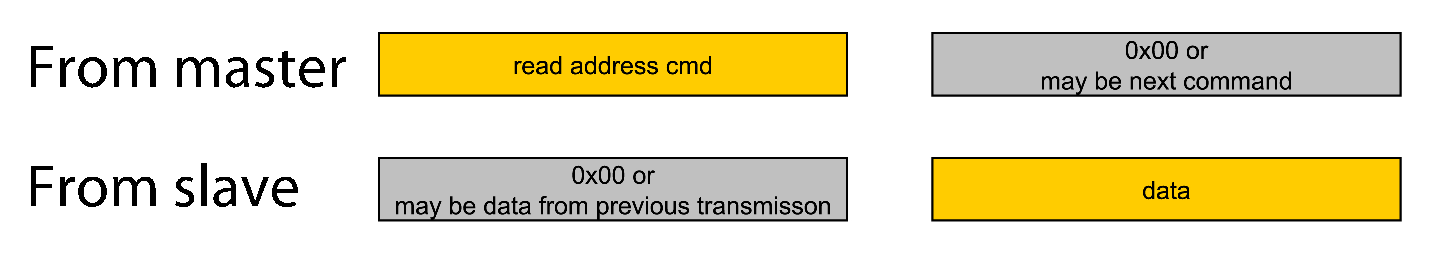
\includegraphics[width=\textwidth]{graphics/spi_protocol_command_structure_read_wlabels.pdf} %trim=l b r t (can cut off from every side)
	\caption{SPI communication when reading from the slave}
	\label{fig:spi_protocol_command_structure_read}			% figure labels are of the form \label{fig:*}
\end{figure}


\subsection{Writing to slave device}
The command send from the master device when writing to the slave device is similar to the one used to read the same address, but with the MSB set to high. The structure of the command byte is shown in figure \ref{fig:spi_protocol_cmd_structure}. Meanwhile the command is send, the slave may be sending the response from last command, or just zeroes if it has nothing to return. Next the master sends the value to be written to the address from the command byte. While the value is send, the output from the slave is just an empty byte. The write sequence is shown in figure \ref{fig:spi_protocol_command_structure_write}.

\begin{figure}[htb]
	\centering
	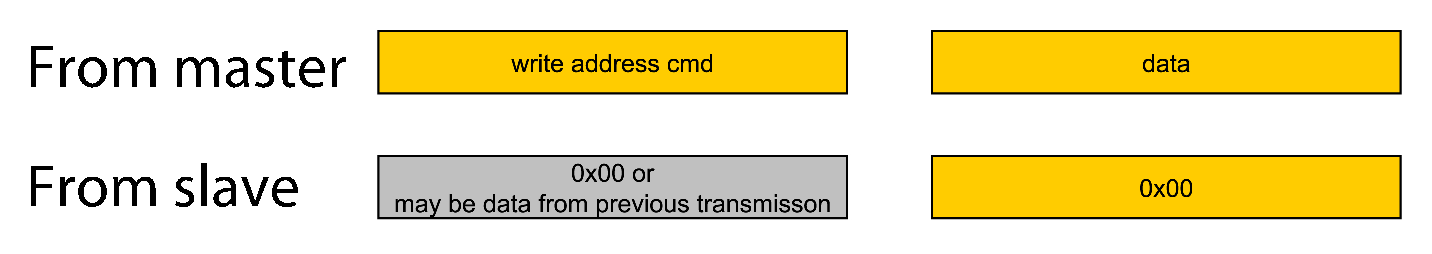
\includegraphics[width=\textwidth]{graphics/spi_protocol_command_structure_write_wlabels.pdf} %trim=l b r t (can cut off from every side)
	\caption{SPI communication when writing to the slave}
	\label{fig:spi_protocol_command_structure_write}			% figure labels are of the form \label{fig:*}
\end{figure}



\section{Protocol ARM implementation}
%\section{Protocol ARM implementation}
One integral part of the project is the communication between the microprocessor and FPGA devices. This section describes the process of implementing SPI communication software (in the remainder of this section just referred to as the \textit{implementation}) on the microprocessor. It will go over the initial demands of the implementation, how it was made, how it works, and how it is supposed to be used (by other parts of the system). A test of the implementation is also described. Finally, the results the test yielded, plus thoughts about further improvements, are discussed.

\subsection{Requirements and delimitations}\label{sec:spi_software_reqs}
The first part of the development process was to specify requirements to the implementation, to make it easier for the rest of the software system to make use of the SPI link. Those requirements were:
\begin{enumerate}
  \item The implementation would have to be multi-task/thread safe, as more than one task may have to use the SPI software interface at any given time.
  \item The interface provided by the implementation should be easy to use by other processes in the system.
\end{enumerate}

To fulfill the first requirement, some problems has to be considered carefully: If more than one task uses the implementations interface to send data asynchronously, how do they receive data back in the correct order? There is only one physical SPI link in the LM3S6965, so it has to be handled by software.
The microcontroller is the exclusive \textit{master} of the SPI link, so only it can initiate communication. The software relies heavily on that fact to facilitate multi-task usage. Also, every time a unit data is sent, the same amount will be received. That way we know, that if a task sends data, the data which is returned immediately afterwards should be directed to that particular task.

The second requirement states that an easy-to-use interface should be provided - in practice through the modules header-file. What is meant with that is, that the user-task should not have to worry about whether or not it is allowed to write to the SPI hardware FIFO at the time it makes a call to the implementation. Additionally, when a task is reading return-data, it should not have to worry about whether it is correctly reading data meant for it, or reading data meant for another task.

Since the whole embedded software system is based on the FreeRTOS real-time kernel, most of the constructs used to implement the SPI communication software, like semaphores and queues, are those provided by the FreeRTOS API.

The documentation of the implementation is split into two parts: One being the interface - the link to the ``outside world'' - and one being the actual transmission and reception to or from the hardware layer FIFO buffers.



\subsection{Interface}
The topmost layer of the implementation is the interface between the SPI implementation and the rest of the program.

The interface quite simply consists of the four functions \texttt{spi\_init}, \texttt{spi\_register\_task}, \texttt{spi\_write\_from\_task} and \texttt{spi\_read\_from\_task}. The \texttt{\_task}-suffix signifies that the function is meant to be called from within a task (and will otherwise have no effect).

The first function to be called under normal circumstances would be \texttt{spi\_init}. It initializes the hardware SPI peripheral for use such as described in [ref freescale etc.]. Also, it creates two tasks; a transmitter and a receiver as well as associated queues and semaphores.

\begin{figure}[htb]
  \begin{subfigure}[b]{0.495\textwidth}
    \centering
    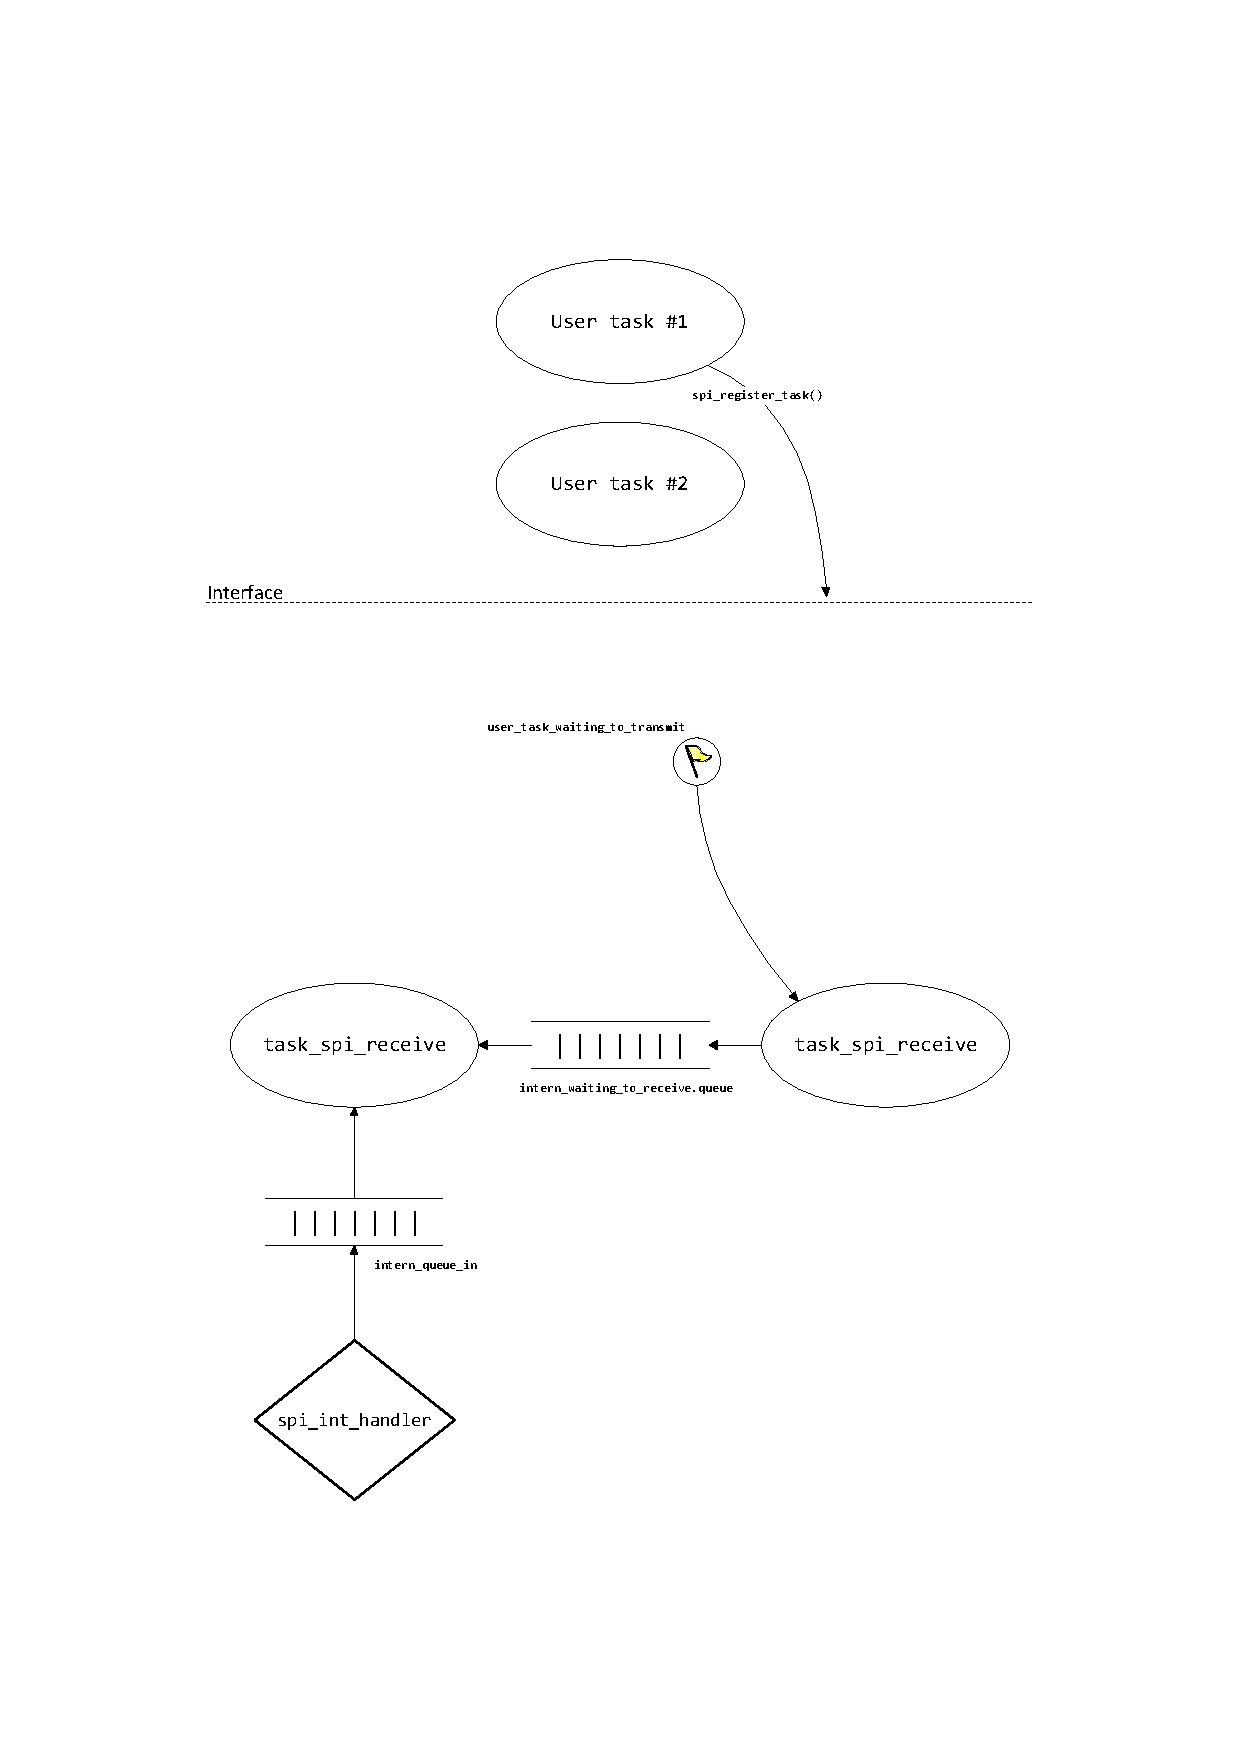
\includegraphics[width=\textwidth,clip,trim=0 0 0 0]{content/04_communication/figures/spi_task_diagram_initial_1.pdf}
    \caption{Before the \texttt{spi\_register\_task} call.}
    \label{fig:spi_task_diagram_initial_1}
  \end{subfigure}
  \begin{subfigure}[b]{0.495\textwidth}
    \centering
    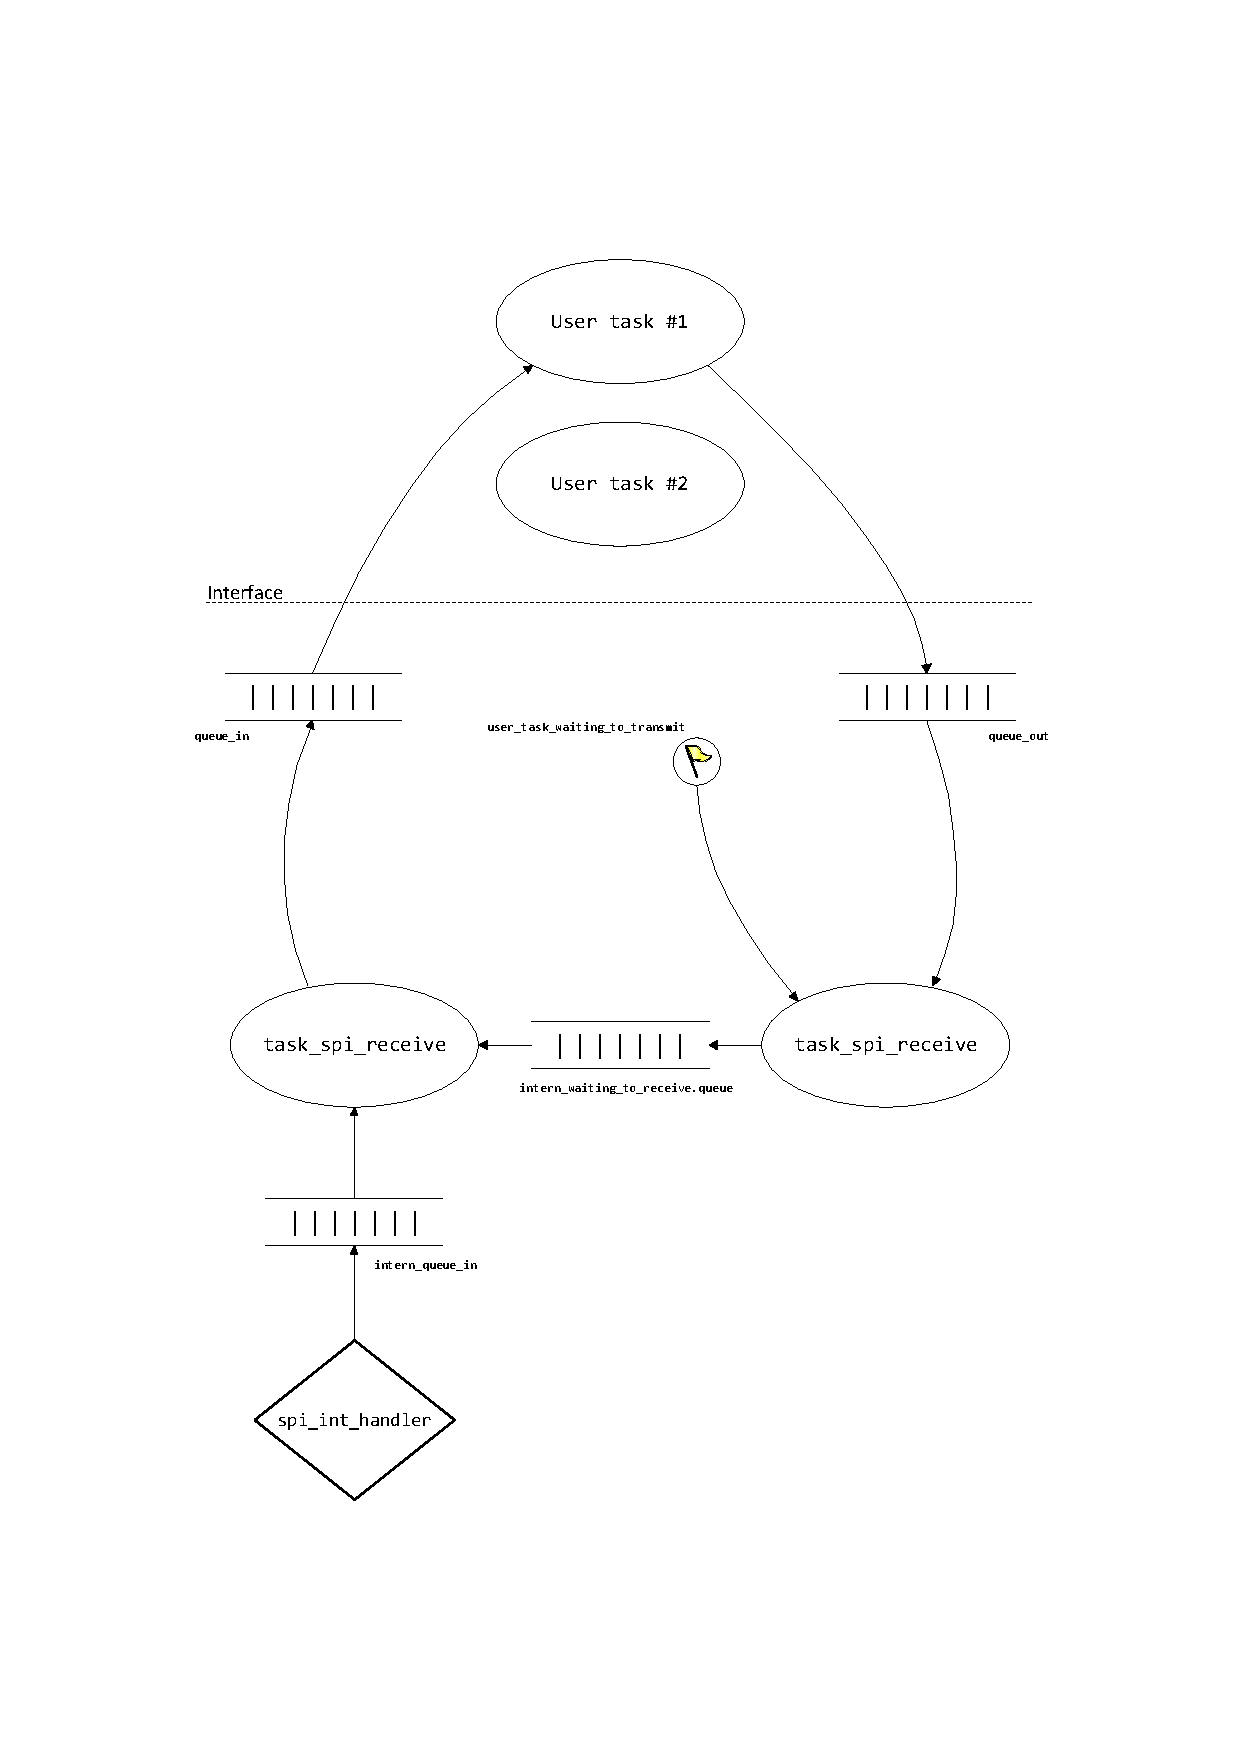
\includegraphics[width=\textwidth,clip,trim=0 0 0 0]{content/04_communication/figures/spi_task_diagram_initial_2.pdf}
    \caption{After the \texttt{spi\_register\_task} call.}
    \label{fig:spi_task_diagram_initial_2}
  \end{subfigure}
  \caption{A user task registering with the SPI interface.}
  \label{fig:spi_register_task}
\end{figure}%trim=l b r t

For at task to be able to use the SPI link, it will have to first make a call to the function \texttt{spi\_register\_task}. That is because resources are allocated dynamically (described in \ref{sec:spi_underthehood}.). Figure \ref{fig:spi_register_task} shows a user task using the register function and getting queues allocated to it. 

When a user task has been successfully registered with the SPI software it is allowed use of the \texttt{spi\_write\_from\_task}- and \texttt{spi\_read\_from\_task}-functions to read and write to and from its private queues. With only those two functions used frequently during runtime, the second design goal is considered fulfilled.

An overview - a task diagram - is shown in figure \ref{fig:spi_task_diagram}.



\subsection{Under the hood}\label{sec:spi_underthehood}
To understand how the implementation works, lets describe what goes on ``under the hood''. That is, between the user interface and the hardware transmit/receive logic. The first design goal was, that the implementation should be thread-safe. To elaborate; the implementation should allow multiple tasks to send and receive data asynchronously. To make that possible, a scheme, where each task gets its own private software buffers for transmission and reception, is used. That way the software implementation can imitate multiple SPI hardware interfaces. The implementation works is such a way that these ``private'' queues are allocated dynamically when a task wishes to use the SPI. The task which wishes to use the SPI is then associated with the queues by task handle.\footnote{A way of uniquely identifying tasks provided by the FreeRTOS API.} The private queues can be seen just below the ``interface line'' on the task diagram in figure \ref{fig:spi_task_diagram}.

\begin{figure}[htb]
  \centering
  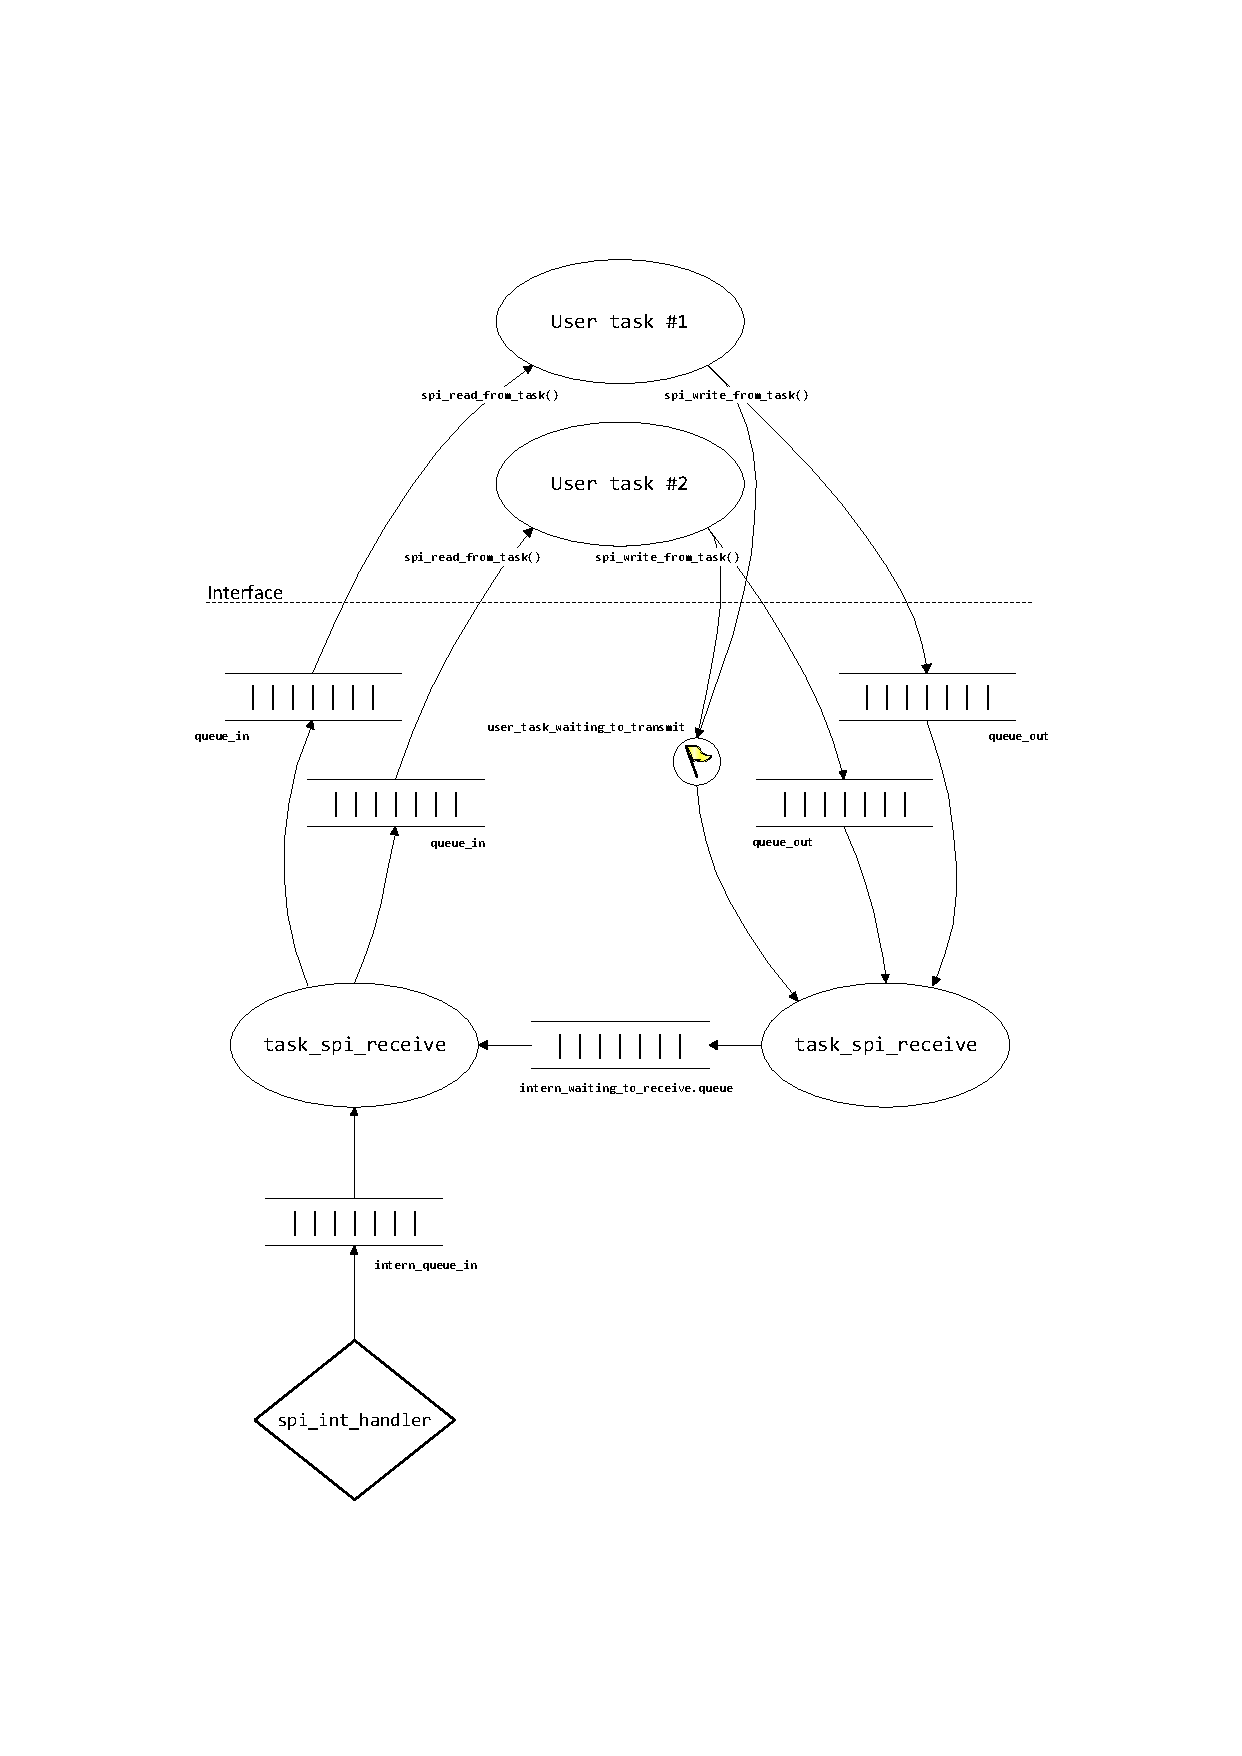
\includegraphics[width=\textwidth,clip,trim=0 15 0 15]{content/04_communication/figures/spi_task_diagram_running.pdf}
  \caption{An overview of the SPI implementation.}
  \label{fig:spi_task_diagram}
\end{figure}%trim=l b r t

A doubly linked list is used to keep track of tasks using the SPI implementation. Each element in the list is a variable that contain the handle of the user task, associated queues and how many units of data they are waiting to receive (after having transmitted). The linked list is semaphore-protected.

Two tasks are used to provide the transmit and receive functionality required: One for transmission and one for reception. When a user task places data in its private transmission-queue, the user task can do no more than to wait for it to appear in its private reception-queue. It is the transmit task's responsibility to make sure the data items get sent, and it is the receiver task's responsibility to direct incoming data to the appropriate tasks reception queue.

Suppose a user task has placed a unit of data in its transmission-queue. At the same time, it must ``give''\footnote{Using FreeRTOS terminology, the functions to unlock resources protected my semaphores are all called \texttt{*SemaphoreGive*}} the binary semaphore \texttt{user\_task\_waiting\_to\_transmit}, which, when given, will un-block the transmit task. This is to avoid having the transmit task spending all of its scheduled time polling the user task transmit queues. When the transmit task is no longer blocked by the \texttt{user\_task\_waiting\_to\_transmit} semaphore, the kernel runs it soon after. When the task runs, it finds a user-task queue which contains items to send and places those items in the hardware transmit FIFO. At the same time, it saves the number of items sent in the variable contained in the linked list. The order in which different user tasks transmit and receive is kept track of by placing them in the queue \texttt{intern\_waiting\_to\_receive.queue} as shown in figure \ref{fig:spi_task_diagram}.

The receiver task blocks on incoming data which is provided by \texttt{spi\_int\_handler} ISR. When it receives a unit of data, it will look in the \texttt{intern\_waiting\_to\_receive.queue} to determine what task the incoming data is for. The data is then placed in that particular user-tasks receive-queue, which the user-task can read at will, more or less. It must be read frequently enough to keep up with the speed at which it the user task transmits, though.

\nomenclature{ISR}{Interrupt Service Routine}



\subsection{Test}


\subsection{Discussion?}
Pros/cons\\
Possible optimization\\
Is it inefficient?\\
Overhead linearly proportional with amounts transmitted/received?\\
Tasks transmission priority is decided by the order in which they use \texttt{spi\_register\_task()}


\section{Protocol FPGA implementation}
% Something about the memeory interface to the other hardware parts
The SPI client interface on the FPGA needs to written in hardware language. As interface to other components in the FPGA it was chosen to use a true dual port RAM on the xilinx board. The RAM then has the responsibility of avoiding race conditions, and presenting an easy-to-use and known-to-work interface between the components. 
Before getting started writing the actual hardware description code, a block and signal description is made to clarify which parts that is needed, and how the internally communicate. Each block is then written in VHDL\footnote{Very high speed integrated circuit Hardware Description Language} and tested in a simulation test bench to ensure the correct functionality. The great advantage of a test bench is the possibility to quickly visualise both internal and external signals over time. When the hardware is tested to work in the simulation, it can be synthesized and put on the FPGA. On the FPGA it is tested with SPI hardware that is known to work. This will make it easier to isolate and debug errors.

\subsection{Hardware planning}
Before writing any code for the SPI hardware, a diagram of the needed hardware blocks were made. A goal when designing the hardware was to make it modular, so parts could be taken out and reused in other projects. The developed diagram can be seen on figure \ref{fig:spi_protocol_fpga_blocks_final_design}, where the signals are represented as round shapes, and hardware blocks as squares. 

\begin{figure}[htb] 
	\centering
	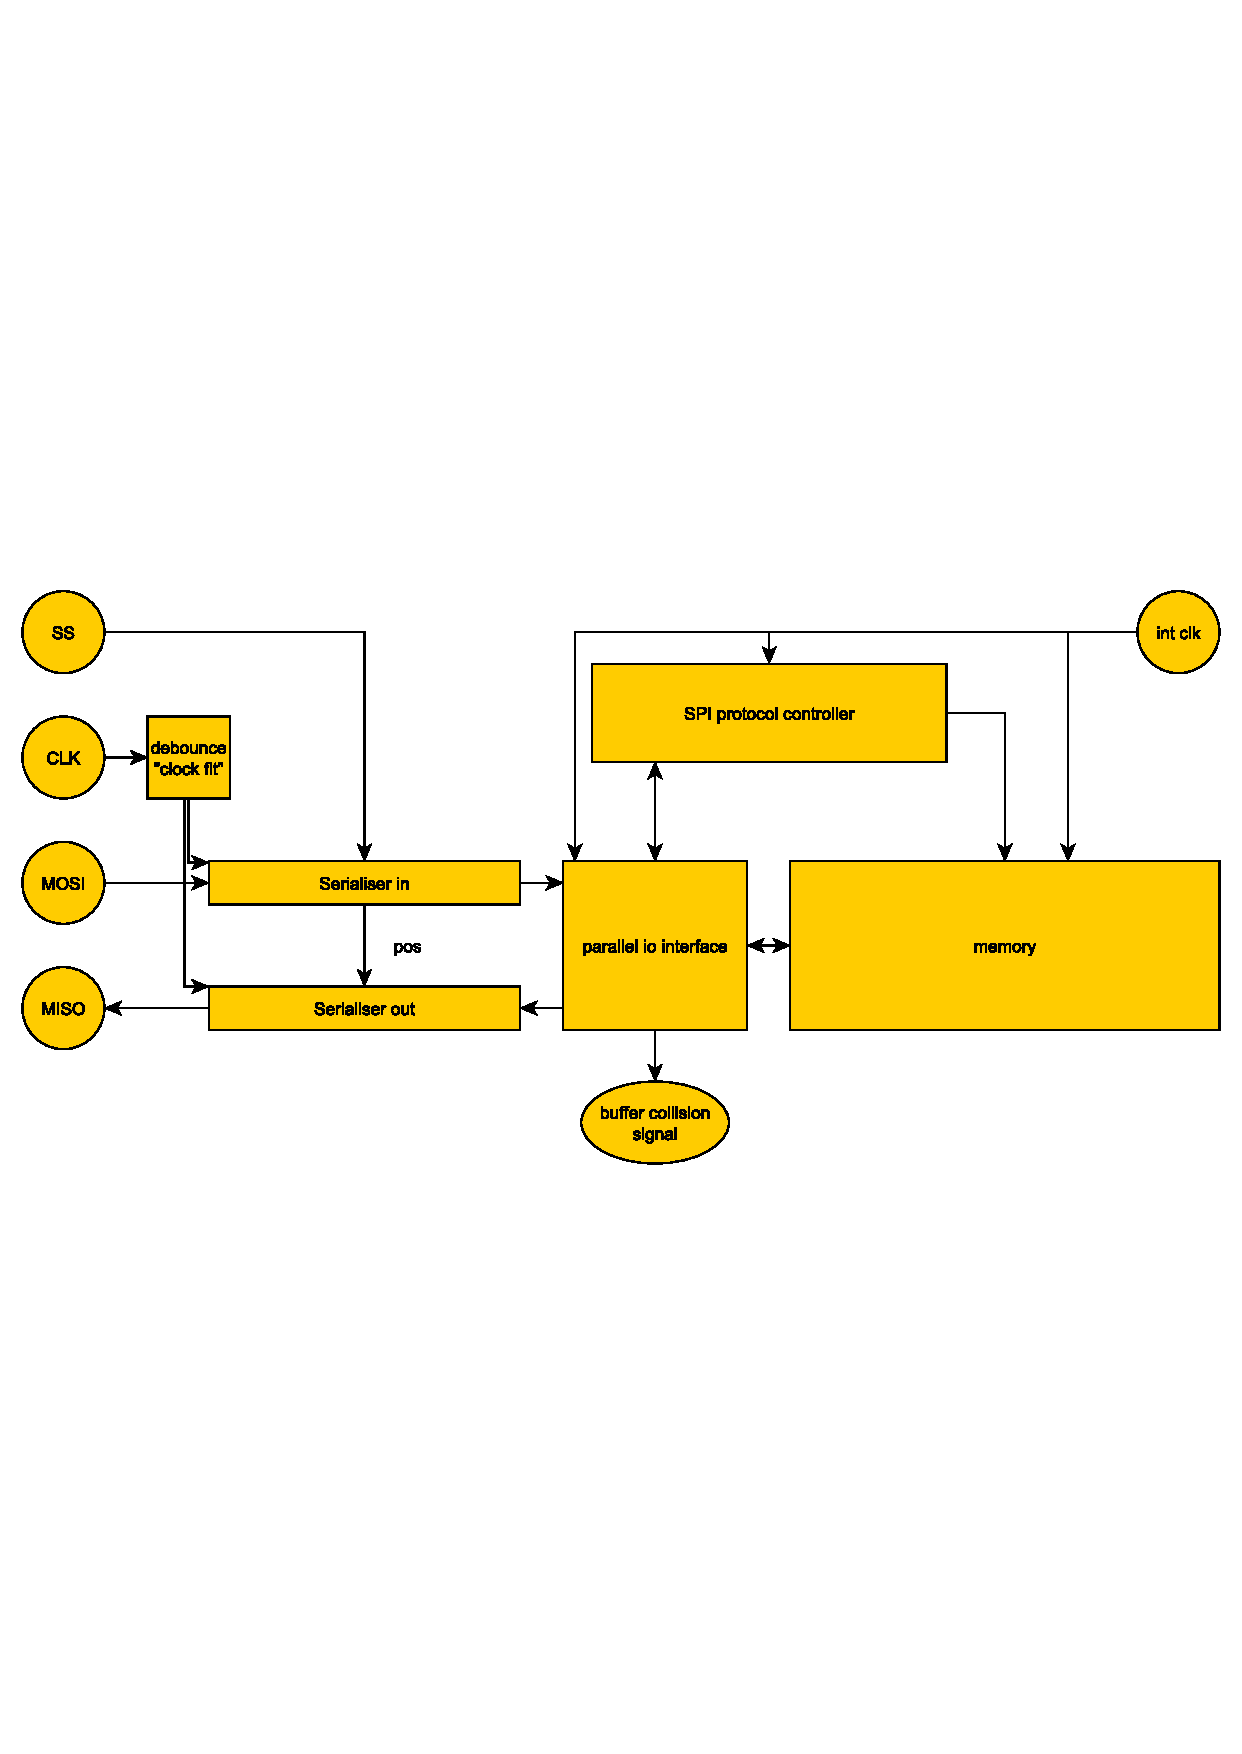
\includegraphics[scale=0.7,trim=0 270 0 270]{graphics/spi_protocol_fpga_blocks_final_design.pdf} %trim=l b r t (can cut off from every side)
	\caption{Blockdiagram for the SPI interface on the FPGA}
	\label{fig:spi_protocol_fpga_blocks_final_design}			% figure labels are of the form \label{fig:*}
\end{figure}

On the figure, the four SPI signals to the ARM board are present to the left, and the memory shared with the other hardware parts implemented on the FPGA to the left.

\subsection{Hardware block description}
The clock debounce process has the purpose of removing noise from the clock signal, and furthermore it can be used to change clock polarity and phase without having to change anything else in the other SPI components.

The MOSI and MISO signals are connected to the two serialiser blocks "Serialiser in" and "Serialiser out". The "Serialiser in" keeps track of the current position in the serialised data, and writes the incoming data to the respective position in the buffer. It can be seen as a demultiplexer where the debounced clock switches to next position in the buffer. When the SS signal is high, the position is always at the starting value. When transmission begins, the SS signal gets pulled low by the master, and the position starts counting accordingly to the pulses from the debounced SPI clock. 

The "Serialiser out" block can be seen as a multiplexer, where the position is fetched from the "Serialiser in" block.

The "parrallel IO interface" process presents an easy to use interface to the serialisers for internal components. It handles the serialiser buffers, and the signals involved in reading and writing from these without race conditions. The interface is made so it is possible to connect other devices then the memory block. This together with the serialisers can be considered the actual SPI hardware. 

The parallel out connections consist of these signals: \texttt{data\_out}, \texttt{data\_out\_valid}, \texttt{data\_out\_ack}\footnote{ack is short for acknowledge} and \texttt{data\_out\_buffer\_collision}. \texttt{Data\_out} and \texttt{data\_out\_ready} are output signals. When the \texttt{data\_out\_valid} is set high, the data is valid on the \texttt{data\_out} port. After the data is read, the reading device signals this by setting the \texttt{data\_out\_ack} pin to high, and the \texttt{data\_out\_valid} gets pulled low so it is ready to signal next time data is ready. If the data is not acknowledged before the next data arrives, the \texttt{data\_out\_buffer\_collision} is pulled high to warn that an internal buffer was not emptied and data was possible thrown away.

The parallel in connections works in a similar way. It consists of three signals: \texttt{data\_in}, \texttt{data\_in\_ready} and \texttt{data\_in\_ack}. When data is to be written to the SPI master, it is set on the \texttt{data\_in} port and the \texttt{data\_in\_ready} is pulled high. When the \texttt{data\_in\_ack} is set high, the data is read and the \texttt{data\_in\_ready} should be pulled low.

The SPI protocol controller has the purpose of determining how to respond to the data received on the serialser, and control the memory accordingly. The basics of the controller is a state machine which is described in \ref{spi_protocol_controller}.

As memory a true dual port ram is used, which is out-of-the-box solution from Xilinx. This RAM has two interfaces, which makes it ideal as interface between communication and other hardware block in the FPGA. The data in and data out ports are connected to the parallel interface and the write and enable signals are connected to the protocol controller. The reading and writing process of the memory module is well described in the datasheet ~\cite{XILINX_MEM}.

\subsection{SPI protocol controller}
\label{spi_protocol_controller}
The "SPI protocol controller" is the state machine which controls the package flow according to the protocol. It has access to read the received data from the parallel interface and sets the control signals both on the parallel interface and the memory block. When data is ready on the parallel interface it is read by the protocol controller and a decision is made about how to respond. The states of the state machine is visualised in figure \ref{fig:spi_protocol_controller_prettystates}.


\begin{figure}[htb] 
	\centering
	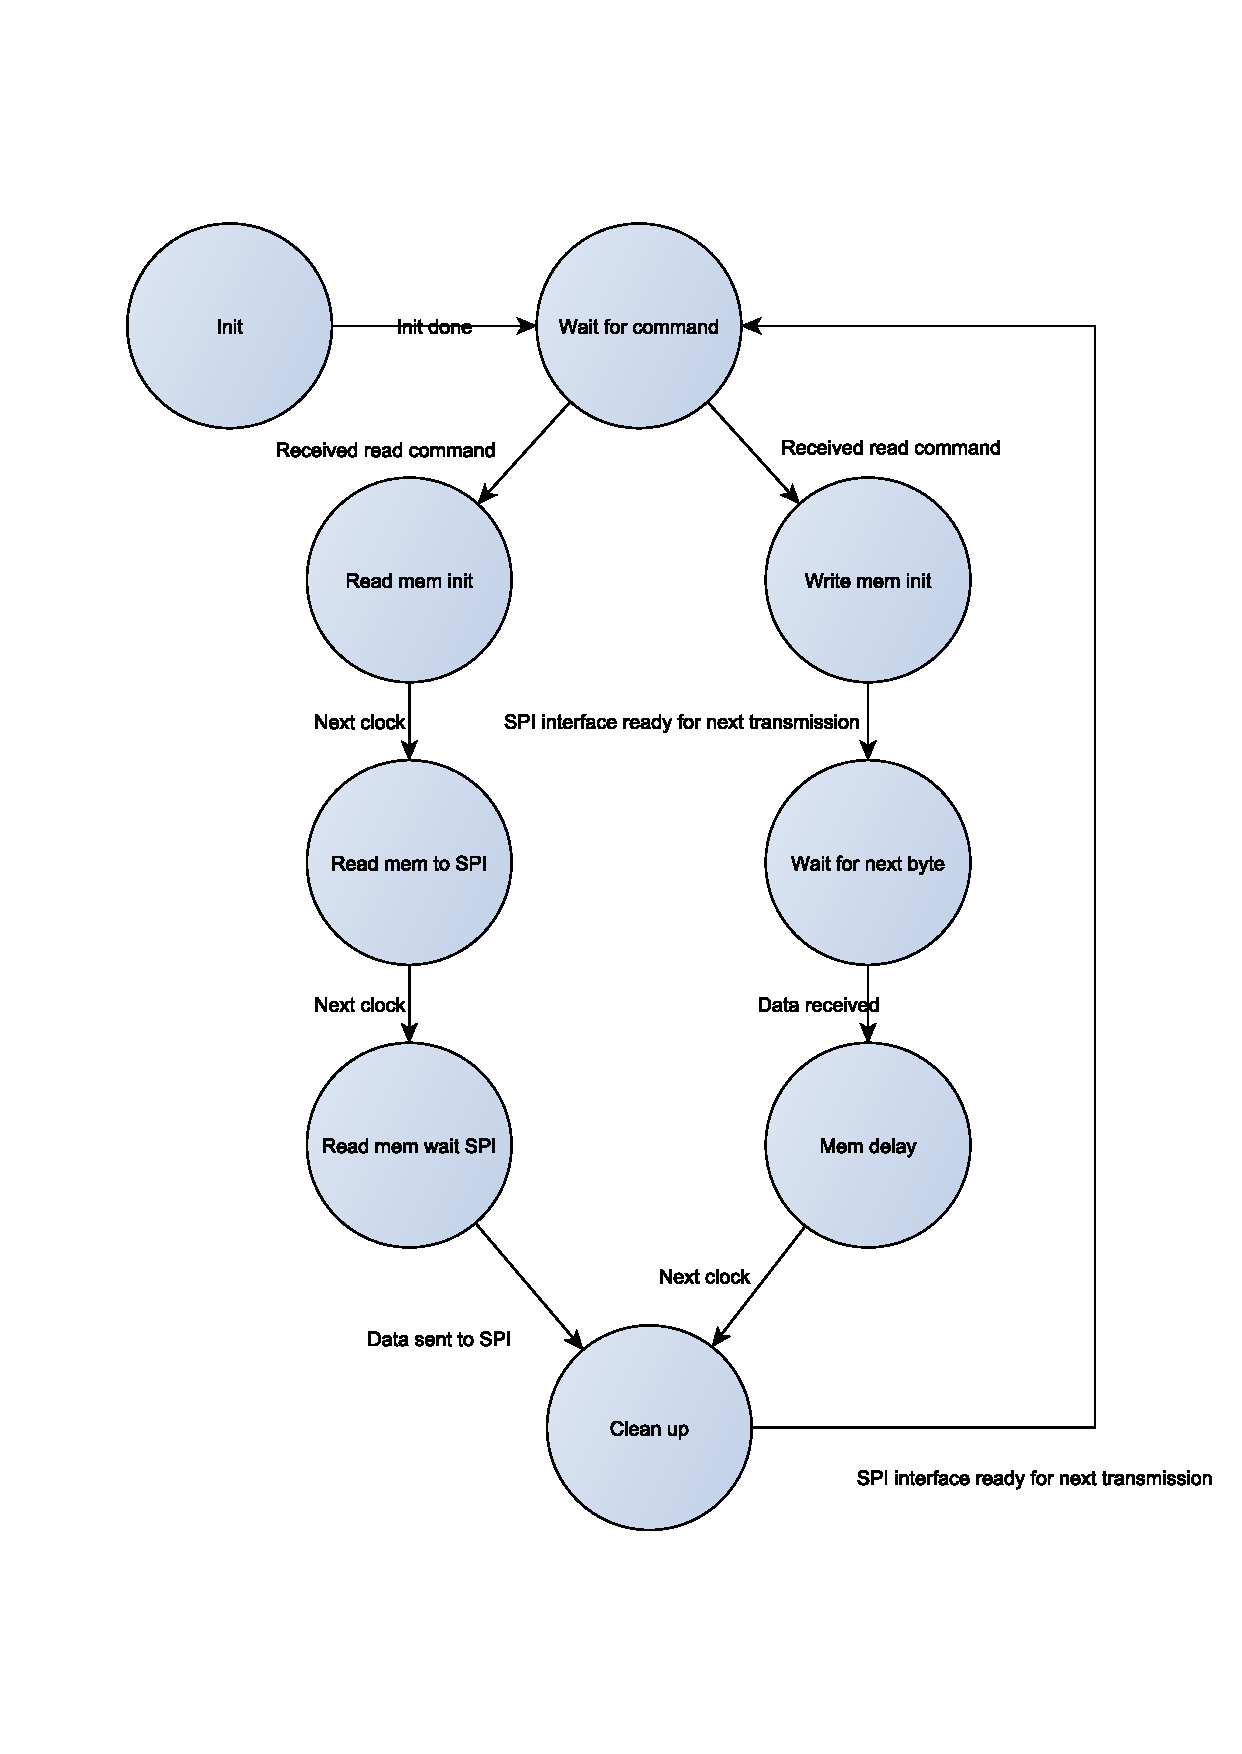
\includegraphics[scale=0.6,trim=0 100 0 100]{graphics/spi_protocol_controller_prettystates.pdf} %trim=l b r t (can cut off from every side)
	\caption{State diagram for the SPI protocol controller}
	\label{fig:spi_protocol_controller_prettystates}
\end{figure}


%\begin{description}
%\item[Init] is the initial state, where it sets up the signals between the SPI and RAM to be ready. When the signals are set, it goes to "Wait for command" state.
%\end{description}

The protocol controller is started in an initial state, where it sets up the signals between the SPI and RAM to be ready. When the signals are set, it goes to a waiting mode, where it will wait for the \texttt{data\_out\_ready} to be set high. When this happens, the data/command is read and the next state depends on whether is was a read or write command.

It the received command was a read command, the next state "Read mem init" will set the requested address on the memory block, and continue to the next state "Read mem to SPI", where the \texttt{data\_out\_ready} will be set on the SPI interface. This will signal the SPI to read from mem and protocol controller will continue to the next state "Read mem wait SPI". In the "Read mem wait SPI" state, it waits for the SPI to acknowledge the data. When this is received it continues to the "Clean up" state, where waits for the SPI interface to be ready for next transmission, and returns back to the "Wait for command" state.

Another possible way through the states in the state machine, is that a write command was received in the "Wait for command" state. When the write command is received the requested write address is set on the memory block and continues to the "Write mem init" state. In the "Write mem init" state it waits for the \texttt{from\_spi\_valid} to go low, so the SPI is ready to receive next transmission. Next it goes to the "Wait for next byte" state, where it waits for the \texttt{from\_spi\_valid} to go high again, which will happen when the next transmission occur. Now it will set the "write" signal high on the memory, so the data will be saved to RAM. It then goes to the state "Mem delay" where it set the "write" signal low again, and continues to the "Clean up" state.
%Scaleability


% Block overview / hardware planning
% Block description
% Testbench

\chapter{Operating system}\label{chap:os}


In the project-description it is stated that a microprocessor shall run a user interface, a regulation system and a SPI communication with the FPGA. This system will require the microprocessor to run multiple tasks and thus an operating system is necessary. It has been decided to use the lent ARM microprocessor so the operating system has to be available for this system.

The system has to run in real time to create a reliable environment for the regulation. Thus a RTOS have to be used.

The group have decided to use FreeRTOS both because it meets the requirements and is well documented, but also because the whole group have experience with FreeRTOS from the EMP course.

\section{ Pre-emptive Scheduling }

To secure that the specific tasks is run in real time pre-emptive scheduling will be implemented. This is implemented by giving tasks priority when they are declared. Thus all tasks which have to run in real time is given a high priority. If a task is scheduled to run, but a task is already running, new task has a higher priority it can temporarily stop the task. Run it's own task and resume the suspended task. That way a high priority task can be guaranteed to run at specific frequency or at certain interrupts.

\section{ Delays  }

In the system tasks does either need to be blocked by a timer or an i/o port. In FreeRTOS the time delay is handled by to different calls. 

To secure that tasks run regularly each task is blocked with either $vTaskDelay$ or $vTaskDelayUntil$. These calls will insure a relatively or a precise frequency of operation respectively. $vTaskDelayUntil$ is able to do this by the user saving current tick at resume-time and giving that as input to the function.
 
\section{ Semaphores }

To synchronize processes and avoid race conditions, FreeRTOS use semaphores. The standard semaphore for synchronization between tasks is a binary semaphore. In FreeRTOS semaphores is created by, like with tasks first creating a handler, using the function $( xSemaphoreHandle xSemaphore )$

The FreeRTOS semaphore have two operations just like standard semaphores, the $wait()$ and $signal()$. They are designed as $xSemaphoreTake$ and $xSemaphoreGive$, respectively. The $xSemaphoreTake$ checks if the semaphore is free and takes it if possible.
When obtained a semaphore can be released with $xSemaphoreGive$.

\section{ Queues }

In FreeRTOS queues are implemented as a mean for intertask communication. It works as an FIFO buffer where the different tasks can either push or pop from the buffer.

\section{ Suspend }
It is also possible to suspend and resume tasks by function calls. If a task is suspended it will not get any CPU time independent of it's priority.

\section{Risks of faults}

FreeRTOS does not do any work for error prevention. Does it is up to the developer to 

Is there a possibility of 
Data corruption
Deadlocks
Priority inversion
\chapter{User interface}\label{chap:ui}
\chapter{Experiments}\label{chap:experiments}
\chapter{Motor Interface testing} \label{sec:llctest}
Each sub block in motor interface section is encapsulated in a separate module.
Each module is tested separately before being assembled in the main memory interface block, and this chapter will deal with the individual module tests, as well as the final test.
The test consists of a testbench file and an associated evaluation.

\section{PWM generator}
This is a test of the PWM module.\\
File: PWMv1.vhd\\
Testbench: pwmtester.vhd
\subsection{Range}
This is a test of the following: Can a duty cycle be set, and will it produce a corresponding correct output?
If the input is all zero or max value, will the module output dc ?
\subsection{Test setup}
The Generator is applied an integer and clock signal as input, the output is plotted. The input integer is slowly incremented.
\subsection{Result}
The observed duty cycle was consistent with the input.
\subsection{Conclusion}
The PWM generator can correctly generate a duty cycle based on the input.



\section{Signed to magnitude}
This is a test of the signed to magnitude splitter.\\
File: SignedToMagnitude.vhd\\
Testbench: signtest.vhd

\subsection{Range}
This test will verify whether the block outputs a correct output based on its input.
\subsection{Test setup}
The block is applied every 16 bit integer combination, and the output is compared.
\subsection{Result}
Every single output matches the input in magnitude, except the largest negative number, which is truncated to the largest positive number.
\subsection{Conclusion}
The block correctly decodes the sign and magnitude, and therefore meets its requirements.

\section{Control block}
This is a test of the top motor control block.\\
File: ControlBlockTop.vhd\\
Testbench: motor\_control\_block\_test.vhd
\subsection{Range}
This test is a test of the control blocks ability to generate the correct control signals based on torque input. Also whether the block correctly reacts to freerun commands.
\subsection{Test setup}
The block is applied an input number which slowly increases from the lowest possible to the larges possible value, the free run bit is toggled after a long time period and the output is plotted.
\subsection{Result}
The block produces a duty cycle corresponding to the magnitude of the input, the output pin of the PWM signal corresponds to that of the sign of the input number. The freerun bit completely shuts off the output and switches the enable pin.
\subsection{Conclusion}
The control block meets the design requirements and works as intended.

\section{Input filter}
This is a test of the input signal filter.\\
File: Hysteresis.vhd\\
Testbench: inputfiltertest.vhd
\subsection{Range}
This tests the input filters ability to remove a high frequency noise signal from the input signal.
\subsection{Test setup}
A correct low frequency signal and a high frequency noise is mixed together and applied to the filter. The output is plotted.
\subsection{Result}
The high frequency signal is removed, and the low frequency signal is slightly delayed.
\subsection{Conclusion}
The filter correctly removes high frequency noise.

\section{Quadrature decoder}
This is a test of the quadrature decoder block.\\
File: FourXDecoderV2.vhd\\
Testbench: decoder\_v2\_testb.vhd
\subsection{Range}
This is a test of the decoders ability to track a position based on quadrature encoder output.
\subsection{Test setup}
The decoder is applied two pulse trains 90 degrees out of phase, corresponding to an ideal encoder output. The output number is plotted.
\subsection{Result}
The decoder counted up for each change in the input signal.
\subsection{Conclusion}
The decoder can correctly track a position.

\section{Velocity estimator using secant method}
This is a test of the first of the two velocity estimators, using the secant method.\\
File: dxdt.vhd\\
Testbench: velocity\_test\_secant.vhd
\subsection{Range}
This test measure the ability of the estimator to give a velocity based on an increasing position.
\subsection{Test setup}
An integer is applied to the input, which is slowly incremented. The output is plotted.
\subsection{Result}
The output was mostly random numbers.
\subsection{Conclusion}
The module did not work, as the output did not in any way correspond meaningfully to the input.

\section{velocity estimator avg}
This is a test of the second of the two velocity estimators, using the running.\\
File: dvdtv2.vhd\\
Testbench: velocity\_test\_avg.vhd
\subsection{Range}
This test measure the ability of the estimator to give a velocity based on an increasing position.
\subsection{Test setup}
An integer is applied to the input, which is slowly incremented. The output is plotted.
\subsection{Result}
The output was mostly random numbers.
\subsection{Conclusion}
As with the previous estimator, the module did not work, as the output did not in any way correspond meaningfully to the input.

\section{Watchdog}
This is a test of the watchdog block.\\
File: watchdog.vhd\\
Testbench: watchdog\_test.vhd
\subsection{Range}
This test measure the watchdogs ability to correctly maintain an alive signal, based on the given input.
\subsection{Test setup}
The block is applied a constantly changing signal, and after a period a contant signal. The output is plotted.
\subsection{Result}
The block output was high as long as the input was changing. The output fell to low shortly after the input stopped changing.
\subsection{Conclusion}
The watchdog worked as specified.

\section{Motor memory interface}
This is a test of the combined motor interface module.\\
File: Motor\_memory\_interface.vhd\\
Testbench: MMI\_test.vhd + (1\_BLINK.COE)
\subsection{Range}
This final test, will test whether the whole system can correctly read and write to the RAM block, and also act on the read data.
\subsection{Test setup}
An input signal is applied to all of the used pins of port JC, in a manner imitating a real signal that would be found in the actual test setup. Also a memory image with velocity commands are loaded in the ram block.

\subsection{Result}
A pwm signal on the output pins is observed, and position/velocity data is recorded in the RAM block.
\subsection{Conclusion}
The MMI block functions as expected and can be used in the project.


\section{Performance testing}

\subsection{Precision of the system}\label{subsec:precisionofsystem}
This experiment will test the precision of the complete system with the
parameters found from simulating the system. The parameters can be found in
table \ref{tab:actual_gain_values}

\subsection*{Setup}

The test is performed by fastening a laser pointer on the pan/tilt system. A
board is placed next to the system and two positions where the pointer is on the
board are chosen as seen in figure \ref{fig:systemtestsetup}. The laser pointer is placed 180 cm
from the board. Thus corresponds to 3cm on the board.

\[ \tan(1 \ deg) \cdot 180 \ cm \approx 3,14 \ cm \]


\begin{figure}[htb] \centering 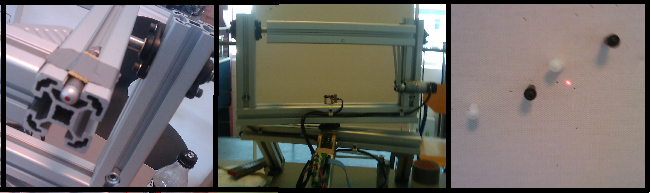
\includegraphics[width=\textwidth,trim=0 0 0
0]{graphics/overallsystemtest.png} %trim=l b r t (can cut off from every side)
	\caption{Setup of the test. From left to right; the mounted laser, the system pointing at the board, laser dot and marks.}
	\label{fig:systemtestsetup}			% figure labels are of the form \label{fig:*}
\end{figure}

The system runs in automode and changes between two setpoints. The positions
are marked and the test ends after ten iterations. 

\subsection*{Results}

At both points the error was less than 5 cm and most of the time
less than two centimetres. This means that the system have an accuracy between 0.658 and
3.293 degrees.

\[ \frac{2,0 \ cm}{3,14\ cm/deg} = 0,64 \ deg \]

\[ \frac{10,0 \ cm}{3,14 \ cm/deg} = 3,19 \ deg \]

\subsection*{Conclusion}

The system itself, has a precision of one third degree.
\[ \frac{360 deg}{1080 tick} = 1/3 deg/tick \]

It is a high precision that have been observed, at times the uncertainty is as
small as the precision of the system. Though it does also show that a higher
precision can be obtained. Overshooting was though occurring in the control.
Additional tuning of the parameters might enhance the performance.

\subsection{Precision of new parameters}\label{sec:precisionofsystem2}

This experiment will test the PID values found in table \ref{tab:actual_gain_values}
under best performance.

Here the system will run in automode between two position but only one of the
positions are marked. 

\subsection*{Setup}

The setup is similar to the setup in section \ref{subsec:precisionofsystem}, see
Figure \ref{fig:systemtestsetup}, with the exception that only one point is measured and the distance to the board is increased to 370 cm. Thus each degree compares to 6,46 cm. This is repeated ten times.

\[ \tan(1 \ deg) \cdot 370 \ cm \approx 6,46 \ cm \]

\subsection*{Results}

In this test the precision of the pan and tilt were recorded to be different. The vertical precision was 7,5 cm, but the horizontal precision was just 2,0 cm. Thus the pan/tilt system have
reached precision of respectively 0.31 degrees and 1.16 degrees.


\[ \frac{2,0}{6,46} = 0.31 \]

\[ \frac{7,5}{6,46} = 1.16 \]

\subsection*{Conclusion}
The pan has reached a constant precision on par with the system precision
of one third of a centimeter. The tilt part has also become adequately precise, but
it should be possible to make it perform even better. It could be that because the
tilt is affected by gravity it is harder to control than the pan.



\section{PID experiments}\label{sec:pid_experiments}
Since adjusting the PID gain values is a somewhat empiric process, the
observations are described in the following as multiple tests although they were
done consecutive.

\subsection{Adjusting the P-gain}\label{sec:pid_experiments_p}
The purpose of this test is to find suitable values for the P-gain and to verify
the values found in simulation.

\subsection*{Setup} The test was performed using the setup described in
\ref{subsec:precisionofsystem}. The system is given two positions and runs in
automode between them. First the P-gain was increased until the system became
unstable, in this test meaning unable to come to rest at the given position.

\subsection*{Results} From \ref{eq:conv} the gains found in simulation can be
converted to the actual system and be compared to the results. The converted
values can be seen in \ref{tab:actual_gain_values}. At P-gain of 600 the gear
belts of the system starts to notch over teeths, while still being stable, so
testing at higher gains were omitted.

It was observed that the system has difficulties reaching
the goal position. This is due to the error becoming smaller and smaller on
approaching the position. The P-gain values found in simulation worked for the
system.

\subsection*{Conclusion} Testing of the system confirms that the control
algorithm works well and the system tracks the given position. The difficulties
reaching the position suggests an I-term should be added.

\subsection{Adjusting the I-gain}\label{sec:pid_experiments_i}
The purpose of this test is to find suitable values for the I-gain and to verify
the values found in simulation.

\subsection*{Setup} The test was performed using the setup described in
\ref{subsec:precisionofsystem}. The system is given two positions and runs in
automode between them. During the test the P-gain was kept at 20.

First the I-gain was increased until the system became
unstable, in this test meaning unable to come to rest at the given position.

From \ref{eq:conv} the gains found in simulation can be converted to the actual
system and be compared to the results. The converted values can be seen in
\ref{tab:actual_gain_values}. 

\subsection*{Results} 
At I-gain of 4 the gear belts of the system starts
to notch over teeths, while still being stable, so testing at higher gains were
omitted.

The sytem reaches the position, but after the overshoot,
especially the tilt halts for a while. This is due to the integrator being at
minimum when passing the setpoint and therefore it takes a while before the
positive error is summed up to a positive contribution to the input. This
suggests adding a D-term at least to the tilt. The problem is insignificant on
the pan due to the relatively small errors compared to the tilt.

\subsection*{Conclusion} Testing showed that the tracking ability of the system
had substantially increased and the speed has increased especially when close to
the goal. The values found from autotune in the simulation works well, but the
system seems to react fine with even higher values, but a  D-term should be
added to get faster recovery after overshoot.

\subsection{Adjusting the D-gain}\label{sec:pid_experiments_d}
The purpose of this test is to find suitable values for the D-gain and to verify
the values found in simulation.

\subsection*{Setup}
The test was performed using the setup described in
\ref{subsec:precisionofsystem}. The system is given two positions and runs in automode between them. During the test
the P-gain was kept at 20 and the I-gain at 2.

First the D-gain was increased until the system became unstable, in this test
meaning unable to come to rest at the given position.

From \ref{eq:conv} the gains found in simulation can be converted to the actual
system and be compared to the results. The converted values can be seen in
\ref{tab:actual_gain_values}. 

\subsection*{Results}
At D-gain of 90 the system becomes unstable.

The D-gain values obtained from simulation worked fine, but it takes a couple of
seconds to finetune into position.

\subsection*{Conclusion}
The PID-regulator now works well and is able to reach a given position. Some
fine-tuning is needed to get perfect parameters.

\begin{table}[htb]
	\begin{center}
	\begin{tabular}{l|c|c|c}			
	Term & Simulation autotune & Measured maximum & Best performance  \\	\hline								
	P-gain pan & 36,25 & 600 & 40 \\
	P-gain tilt   & 18,50 & 600 & 20 \\
	I-gain pan  & 0,78 & 4 & 1,5 \\
	I-gain tilt   & 0,40  & 4 & 0,5 \\
	D-gain pan & 78,25 & 90 & 0,5 \\
	D-gain tilt   & 40,50 & 90 & 2 \\
	\end{tabular}
	\end{center}
	\caption{P-gain values converted to be used in the control algorithm and the values measured on the system}				
	\label{tab:actual_gain_values}			
\end{table}

\subsection{Tuning the PID parameters}
The purpose of this test is to increase the accuracy of the system by changing
the drive belt and retune the parameters of the PID.

\subsection*{Setup}
The test was performed using the setup described in \ref{subsec:precisionofsystem}. The
system is given two positions and runs in automode between them while tuning the
parameters of the PID.

\subsection*{Results}
The drive belt on the pan was replaced.

The PID parameters were tuned slightly, reducing the D-gain and increasing the
I-gain to obtain better precision. The new values can be found in
\ref{tab:actual_gain_values} under best performance. Small changes were made to
parts of the control algorithm concerned with evaluating when the position is reached.

The precision of the system was raised to a level where this test can no
longer be used to measure the inaccuracy. 

A periodic error was observed as the small drive wheel on the motor sometimes
jumps a tooth and after a while jumps back. The belt seems fine, but
the teeths of the drive wheel is worn

\subsection*{Conclusion}
The performance of the system has been gratly improved and new tests should be
performed with greater distance between the pan-tilt and the board. 

If the error with the drive belt continues, the drive wheel should be replaced.


\subsection{Verification of the control frequency}
The purpose of this test is to verify that the control task actually runs at 100 Hz.

\subsection*{Setup}
At the entry of control task a pin is set, and at the end of the control task it
is cleared. An oscilloscope is connected to the pin. While the system is running, the period between rising edges is measured using the oscilloscope.

\subsection*{Results}
The results vary between 9,80 and 9,90 ms. This is equal to between 101,01 Hz and 102,04 Hz, meaning an error of less than 2 percent.

\subsection*{Conclusion}
The control task runs close to 100 Hz and therefor jitter should not be a problem.










\chapter{Discussion}\label{chap:discussion}
The main approach in this project, has been to divide the assignment into specialized manageable tasks, with defined interfaces.  This has given each member of the group a chance to specialize in their given assignment area, without the need to worry about the larger picture of the project.

In this project, no practical application, fx a tracking system, was to be implemented using the system.
This made it the scope of this project to build an interface, to show the efficiency of the control system. Thus it was not possible to define all the systems requirements.

In contrast with previous projects, where the group have attempted to use responsibility based work models, specifically the Belbin model, this time an expertise focused model was used, where each individual group member primarily focused on their own practical field, and all other assignment were handled as they came naturally. 

Instead of having a lot of meetings, the group used a central log. This was an open Google document, where most of the  group communication took place. This freed up a lot of time, that would otherwise have been spent on meetings for the sake of coordination. And thus time could be, and was, used more constructively. The log could also guaranteed that each group member quickly could get a clear picture of the status of the project, and what small assignments were pending.

Even though the project resulted in a successful system, there have been several areas where improvements could be made. For instance the velocity estimators on the FPGA, together with the control model that used them.
Also some of the initial solutions proposed, turned out to be more than sufficient, but hard to implement, and therefore a simpler solution was implemented. The statespace model was proposed in the simulation chapter, but it ended up with a simple S-domain transfer function. These areas were all explored a bit, but was ultimately cut, due to the fact that it was prioritized to have a working system by the deadline, instead of a non working, but more advanced system.

Due to the architecture of the system having an extremely low coupling, additions and replacements could be easily made and interfaced, without requiring a complete redesign. The test of the CPU load also shows that a more complicated control algorithm could be implemented without requiring new hardware, or redesign of other modules.

test vs debug

arbejdsform
	forventninger: krav til 
	project forløb


pony

\chapter{Conclusion}\label{chap:conclusion}
% 
% References
\clearpage
\nocite{*} % Includes all of the .bib content
\printbibliography\addcontentsline{toc}{chapter}{Bibliography}
%
% Appendix
\appendix %all sections below are numbered A, B, C,...
\chapter{Calculations for dynamics}\label{app:dynamics_calc}
This appendix will contain calculations for the chapter concerning dynamics of the system.

\section{Inertia of the pan/tilt}
A sketch of the pan/tilt system is shown in the figure below.
\begin{figure}[htb]
	\begin{center}
	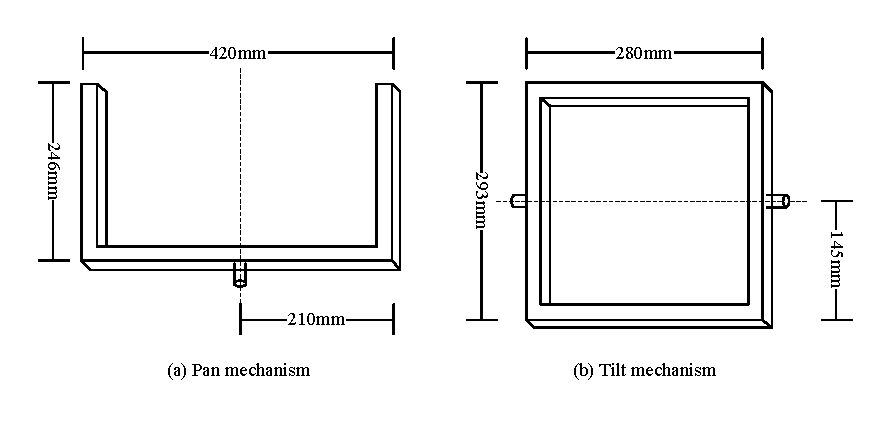
\includegraphics[scale=1,trim=0 0 0 0]{graphics/pan_tilt_sketch.pdf} %trim=l b r t (can cut off from every side)
	\caption{Simple sketch of the pan/tilt system with measurements. The dimension of the profile is 40 x 40 mm. The profile that is used weigh $1.565\sfrac{kg}{m}$}
	\label{fig:pan_tilt_sketch}			% figure labels are of the form \label{fig:*}
	\end{center}
\end{figure}

\subsection{Pan inertia}
To calculate the inertia of the pan mechanism some considerations have to be made about how to model it. Figure \ref{fig:pan_tilt_sketch}(a) will be modelled in a way so the bar connected to the turning shaft will be considered as a rod with two point masses connected to each end of the bar, the total inertia of the pan mechanism will be calculated from the parallel axis theorem. The parallel axis theorem says:
\begin{equation}
	J = J_{COM} + M d^{2} \label{eq:parallel_axis_theorem}
\end{equation}
where $J$ is the total inertia, $J_{COM}$ is the inertia of the base bar, $M$ is the mass that is displaced and $d$ is the displacement. $J_{COM}$ is calculated as follows:
\begin{equation}
	J_{COM} = \dfrac{M L^{2}}{12} \Longrightarrow J_{COM} = \dfrac{(1.565\sfrac{kg}{m} \cdot 0.42m) \cdot (0.42m)^{2}}{12} = 0.058 kg \cdot m^{2}
\end{equation}
Calculation of the total inertia is calculated as follows:
\begin{align}
J_{Pan} &= J_{COM} + 2 \cdot M d^{2} \Longrightarrow \\
J_{Pan} &= 0.058 kg \cdot m^{2} + 2 \cdot (1.565\sfrac{kg}{m} \cdot 0.246m) \cdot (0.21m)^{2} \Longrightarrow \label{eq:pan_inertia_temp} \\ 
J_{Pan} &= 0.092 kg \cdot m^{2}\label{eq:pan_inertia}
\end{align}
\ref{eq:pan_inertia_temp} has its second term multiplied with two, this is done as the pan mechanism has two masses that is displaced equally from the axis of rotation.

\subsection{Tilt inertia}
The inertia of the tilt part of the system is considered as a rod with two point masses displaced equally from the axis of rotation. The inertia is calculated the following way:
\begin{equation}
	J_{COM} = \dfrac{ML^{2}}{12} = \dfrac{2 \cdot 1.565 \sfrac{kg}{m} \cdot 0.293 m \ (0.293m)^{2}}{12} = 0.079 kg \cdot m^{2}
\end{equation}
Adding the displaced masses to the inertia is done with the parallel axis theorem as follows:
\begin{align}
J_{Tilt} &= J_{COM} + 2 \cdot M d^{2} \Longrightarrow \\
J_{Tilt} &= 0.079 kg \cdot m^{2} + 2 \cdot (1.565\sfrac{kg}{m} \cdot 0.280m) \cdot (0.145m)^{2} \Longrightarrow \label{eq:tilt_inertia_temp} \\ 
J_{Tilt} &= 0.097 kg \cdot m^{2}\label{eq:tilt_inertia}
\end{align}

\section{Gears}
The load at the motors are the reflected inertia through the gears plus the inertia of the rotor in the motor, the rotors inertia is omitted. The two gears are connected together and then connected between the motor and the inertia. The gearing system is equal on the pan and the tilt. Figure \ref{fig:app_gears} show a simplification of the gearing.
\begin{figure}[htb]
	\begin{center}
	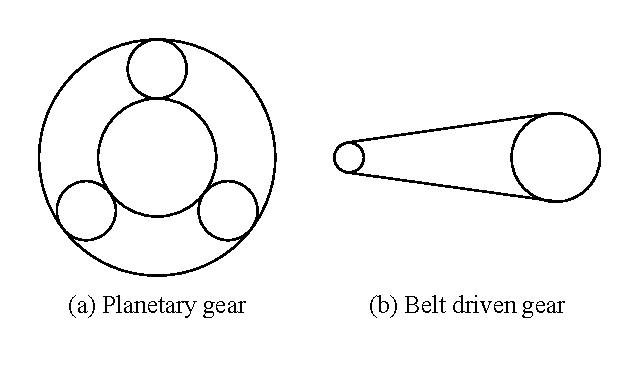
\includegraphics[scale=1,trim=0 0 0 0]{graphics/gears.pdf} %trim=l b r t (can cut off from every side)
	\caption{Simplification of the gears in the pan/tilt system. (a) Show a simplification of a planetary gear which has, according to the datasheet of the motor which is included on the CD, a gearing of $N = 30:1$. (b) The gearing of the belt driven gear is experimental measured and calculated to be $N = 1:3$}
	\label{fig:app_gears}			% figure labels are of the form \label{fig:*}
	\end{center}
\end{figure}
The load reflected through a gear is given by\footnote{REF NEEDED!!!   (http://www.techno-isel.com/tic/h834/PDF/H834P009.pdf)}:
\begin{equation}
	J_R = \frac{J_L}{N^{2}}
\end{equation}
where $J_R$ is the reflected load behind the gear, $J_L$ is the load in front of the gear, N is the gear ratio. As the pan and tilt gearing is equal the following expression is derived the total gearing between the motor and the mass:
\begin{equation}
	J_R = \frac{\frac{J_L}{(\sfrac{1}{3})^{2}}}{30^{2}} = \frac{J_L}{(\sfrac{1}{3})^{2} \cdot 30^{2}}\label{app:eq_reflected_inertia_temp}
\end{equation}

\subsection{Reflected inertia (pan)}
If the inertial load from the pan is substituted into equation \ref{app:eq_reflected_inertia_temp} the following is obtained:
\begin{equation}
	J_{Pan} = \frac{0.092 kg \cdot m^{2}}{(\sfrac{1}{3})^{2} \cdot 30^{2}} = 0.920 \cdot 10^{-3} kg \cdot m^{2} \label{app:eq_reflected_pan_inertia}
\end{equation}

\subsection{Reflected inertia (tilt)}
If the inertial load from the tilt is substituted into equation \ref{app:eq_reflected_inertia_temp} the following is obtained:
\begin{equation}
	J_{Tilt} = \frac{0.097 kg \cdot m^{2}}{(\sfrac{1}{3})^{2} \cdot 30^{2}} = 0.970 \cdot 10^{-3} kg \cdot m^{2} \label{app:eq_reflected_pan_inertia}
\end{equation} 

\chapter{Calculations for control}\label{app:control_calc}

%
\end{document}
